% !TeX program = pdflatex
% Compile with build.ps1. Diagrams use TikZ; the cover logo is in assets/.
\documentclass[11pt,a4paper]{article}
\usepackage[T1]{fontenc}
\usepackage[utf8]{inputenc}
\usepackage[english]{babel}
\usepackage{mathpazo}
\usepackage{amsmath,amssymb,mathtools}
\usepackage{microtype}
\usepackage[a4paper,margin=26mm,headheight=24pt]{geometry}
\usepackage{xcolor,graphicx,booktabs,tabularx,array,longtable}
\usepackage{enumitem,titlesec,fancyhdr,needspace,placeins}
\usepackage[most]{tcolorbox}
\usepackage{tikz}
\usetikzlibrary{arrows.meta,positioning,fit,backgrounds,calc}
\usepackage{hyperref}
\usepackage[nameinlink,noabbrev]{cleveref}
\definecolor{wine}{HTML}{7A1737}
\definecolor{ink}{HTML}{202020}
\definecolor{muted}{HTML}{555555}
\definecolor{pale}{HTML}{F8F3F5}
\hypersetup{colorlinks=true,linkcolor=wine,urlcolor=wine,citecolor=wine,pdftitle={Automatic Verification of Intelligent Systems -- Lecture Notes},pdfauthor={Matt Clifford Trinidad Ramos},bookmarksnumbered=true}
\urlstyle{same}
\color{ink}
\setlength{\parindent}{0pt}
\setlength{\parskip}{5pt plus 1pt minus 1pt}
\linespread{1.06}
\setlength{\emergencystretch}{2em}
\setlist{nosep,topsep=5pt,leftmargin=1.6em}
\titleformat{\section}{\Large\bfseries}{\color{wine}\thesection}{0.65em}{}
\titleformat{\subsection}{\large\bfseries}{\color{wine}\thesubsection}{0.65em}{}
\titleformat{\subsubsection}{\normalsize\bfseries}{\color{wine}\thesubsubsection}{0.6em}{}
\titlespacing*{\section}{0pt}{18pt}{9pt}
\titlespacing*{\subsection}{0pt}{13pt}{5pt}
\titlespacing*{\subsubsection}{0pt}{10pt}{3pt}
\setcounter{tocdepth}{2}
\numberwithin{equation}{section}
\numberwithin{figure}{section}
\numberwithin{table}{section}
\pagestyle{fancy}\fancyhf{}
\fancyhead[L]{\small\textsc{AVIS}}
\fancyhead[R]{\small\nouppercase{\rightmark}}
\fancyfoot[L]{\scriptsize AVIS \enspace / \enspace LECTURE NOTES}
\fancyfoot[C]{\small\thepage}
\fancyfoot[R]{\scriptsize Matt Clifford Trinidad Ramos}
\renewcommand{\headrulewidth}{0.4pt}\renewcommand{\footrulewidth}{0.4pt}
\renewcommand{\headrule}{\hbox to\headwidth{\color{wine}\leaders\hrule height\headrulewidth\hfill}}
\renewcommand{\footrule}{\hbox to\headwidth{\color{wine}\leaders\hrule height\footrulewidth\hfill}}
\renewcommand{\sectionmark}[1]{\markright{\thesection\enspace #1}}
\renewcommand{\subsectionmark}[1]{}
\newtcolorbox{concept}[1]{enhanced,breakable,colback=pale,colframe=wine,boxrule=.45pt,arc=1mm,left=9pt,right=9pt,top=6pt,bottom=6pt,fonttitle=\bfseries,title={#1},colbacktitle=wine,coltitle=white,before skip=9pt,after skip=9pt}
\newtcolorbox{technicalnote}[1]{enhanced,breakable,colback=black!2,colframe=muted,boxrule=.4pt,arc=1mm,left=9pt,right=9pt,top=6pt,bottom=6pt,fonttitle=\bfseries,title={#1},colbacktitle=black!8,coltitle=ink,before skip=9pt,after skip=9pt}
\newtcolorbox{sourcecorrection}[1]{enhanced,breakable,colback=pale,colframe=wine,boxrule=.7pt,arc=1mm,left=9pt,right=9pt,top=6pt,bottom=6pt,fonttitle=\bfseries,title={Source correction: #1},colbacktitle=wine,coltitle=white,before skip=9pt,after skip=9pt}
\newtcolorbox{supplementary}[1]{enhanced,breakable,colback=black!1,colframe=wine!65!black,boxrule=.4pt,arc=1mm,left=9pt,right=9pt,top=6pt,bottom=6pt,fonttitle=\bfseries,title={Supplementary clarification: #1},colbacktitle=wine!8,coltitle=ink,before skip=9pt,after skip=9pt}
\newcommand{\formulanote}[1]{\par\vspace{1mm}{\small\color{muted}\textit{Symbols:} #1}\par}
\newcommand{\source}[1]{\par{\small\color{muted}\textit{Source: #1.}}\par}
\newcommand{\clarify}[1]{\par\textbf{Clarification.} #1\par}
\newcommand{\module}[2]{\clearpage\section{#1}\source{#2}}
\newcommand{\R}{\mathbb{R}}
\DeclareMathOperator*{\argmin}{arg\,min}
\newcolumntype{P}[1]{>{\raggedright\arraybackslash}p{#1}}
\newcolumntype{Y}{>{\raggedright\arraybackslash}X}
\tikzset{process/.style={draw=wine,fill=pale,rounded corners=1mm,minimum height=10mm,text width=24mm,align=center,font=\small},arr/.style={-{Latex[length=2mm]},thick},lab/.style={font=\footnotesize,align=center,fill=white,inner sep=2pt}}
\begin{document}
\hypersetup{pageanchor=false}
\begin{titlepage}
\centering
\vspace*{3mm}
\IfFileExists{assets/sapienza-logo.png}{%
  
\includegraphics[width=85mm,trim=226bp 221bp 225bp 226bp,clip]{assets/sapienza-logo.png}\par
}{%
  {\Large\bfseries\color{wine} SAPIENZA UNIVERSIT\`A DI ROMA}\par
}
\vspace{26mm}
{\color{wine}\rule{\textwidth}{0.6pt}}\\[10mm]
{\LARGE\bfseries Automatic Verification\\[3mm]of Intelligent Systems}\\[7mm]
{\Large Lecture Notes}\\[5mm]
{\large Dynamical Systems, Adaptive Software,\\Optimal Control and LLM Training}\\[10mm]
{\color{wine}\rule{\textwidth}{0.6pt}}
\vfill
{\small\textsc{Course lecturer}}\\[2mm]
{\large Enrico Tronci}\\[12mm]
{\small Department of Computer Science\\Sapienza University of Rome}\\[12mm]
{\small Notes prepared by}\\[2mm]
{\large\bfseries Matt Clifford Trinidad Ramos}\\[12mm]
\vspace*{12mm}
\end{titlepage}
\pagenumbering{roman}\hypersetup{pageanchor=true}
\begingroup\small
\tableofcontents
\endgroup
\clearpage
\section*{Reading guide}\markright{}
\addcontentsline{toc}{section}{Reading guide}
These notes develop the supplied lecture material into a continuous account of modelling, learning, feedback control, and optimal decision making. The source order is preserved: course introduction, adaptive video compression, continuous-time systems, discrete-time systems, continuous-time optimal control, discrete-time optimal control, and LLM training with SFT and reinforcement learning.

\textbf{Scope and attribution.} The course title and lecturer are taken from the introductory deck. Four technical decks are dated September 27, 2026, and the LLM lecture is dated October 1, 2026; no academic year is explicitly stated. The discrete-time systems deck identifies itself as ``Dynamic Systems \& Discrete Modeling'' and uses ``Control Theory'' in its footer, without naming an individual author. It is included as supplied course material without adding an author attribution to that deck.

\textbf{Added lecture and file correspondence.} The current optimal-control uploads, \texttt{1000-\allowbreak opt-\allowbreak ctr-\allowbreak ct-\allowbreak sys.pdf} and \texttt{2000-\allowbreak opt-\allowbreak ctr-\allowbreak dt-\allowbreak sys.pdf}, are identical to the earlier files prefixed \texttt{4000} and \texttt{5000}. Their content is already developed in Sections 5 and 6 and is counted once. Section 7 adds all 15 pages of \texttt{3000-RL4LLM.pdf}. The seven unique decks contain 82 physical source pages.

\textbf{How to read corrections.} The mathematical development follows the slides, with explicitly identified corrections where their equations or claims are inconsistent. Explanatory assumptions and derived intermediate steps make the notes usable independently. In particular, the video-compressor slides contain an incorrect characteristic-polynomial expansion. The corrected derivation is given in \cref{sec:poles}, and the original reasoning is accounted for in \cref{sec:sourcepoles}.

\textbf{Visual provenance convention.} Burgundy \emph{Source correction} boxes mark places where the supplied material is mathematically or technically inconsistent and the correction is derived explicitly. Grey \emph{Technical note} boxes clarify assumptions or interpretation. Light \emph{Supplementary clarification} boxes contain useful context supported by references beyond the supplied lecture decks; they are not presented as additional lecture content.

\textbf{Source references.} Page references denote physical PDF pages, starting at 1. Several slide footers have incorrect totals: the compressor PDF contains 28 pages despite a denominator of 29, the discrete-time systems PDF has 14 pages despite a denominator of 13, and three six-page decks show a denominator of 1. The coverage map in Appendix~\ref{app:coverage} uses the actual pages.

\begin{concept}{Notation conventions}
Continuous time is written as $t$; discrete time is normally $k$. The compressor lecture retains its original discrete index $t$. The symbols $x$, $u$, and $y$ denote state, input, and output; their dimensions are specified locally. The symbol $\lambda$ denotes an eigenvalue in stability analysis and a costate in optimal control. These are different uses. Superscript $T$ denotes transpose, and $Q\succeq0$ ($Q\succ0$) means symmetric positive semidefinite (positive definite).
\end{concept}

\textbf{Study route.} First identify the state and the timing of the input. Next distinguish the model from the measured system. Then ask whether the objective is tracking, stability, or cost minimization. Finally check the assumptions under which the claimed guarantee holds. An accurate model, a stable model, and a stable adaptive implementation are separate assertions.

\clearpage\pagenumbering{arabic}
\section{Course introduction}
\source{1000-intro.pdf, pp.\ 1--7}
\subsection{Identity, logistics, and assessment}
The course is \emph{Automatic Verification of Intelligent Systems}, taught by Enrico Tronci in the Computer Science Department at Sapienza Universit\`a di Roma. The introductory slide gives the departmental address as Via Salaria 113, 00198 Roma, Italy, and the research website \url{https://raise.uniroma1.it/}. Contact: \href{mailto:tronci@di.uniroma1.it}{tronci@di.uniroma1.it}.

The timetable below reproduces the supplied introduction; it is a record of the slides, not an independently verified current timetable.
\begin{center}
\begin{tabularx}{\textwidth}{@{}l l Y@{}}\toprule
Day & Time & Location\\\midrule
Monday & 17:00--18:30 & Room G50, RM115, Building G, E01P03L001; Viale Regina Elena 295, Roma.\\
Thursday & 11:00--13:30 & Same room and address.\\\bottomrule
\end{tabularx}
\end{center}
Course material and recordings are provided through \url{https://elearning.uniroma1.it/}. The list includes the syllabus, slides, books, software, videos, and old exams. The registration instruction explicitly names the \emph{Software Verification} course on that platform. This wording is preserved as a source ambiguity: it differs from the title of this course.

\begin{concept}{Assessment stated in the introduction}
The written examination contributes 50\% and the software project contributes 50\%. A mark of at least $18/30$ is required in \emph{each} component; a passing weighted average alone is insufficient.
\end{concept}

\subsection{Learning objectives}
The first objective is to develop modelling ability for the formalization of requirements, design, and Verification and Validation (V\&V) of intelligent systems. A model should make the relevant assumptions, behaviours, and desired properties explicit enough for analysis.

The second objective is to understand the mathematical tools that enable the design and analysis of these systems. The third is to know software tools that support automatic design and analysis. The fourth is research-oriented: acquiring the knowledge needed to design algorithms that advance the state of the art in automated design and analysis of intelligent systems.

The following case study connects these objectives: a software controller learns an environment model online and adapts its decisions using a mathematically analysed feedback law. The final introductory slide is a closing acknowledgement and introduces no additional academic content.

\module{An intelligent system: adaptive video compression}{1500-video-compressor.pdf, pp.\ 1--28}
\subsection{Problem and quality objective}
The case study concerns sending video frames, such as JPEG images, over the Internet. Compression reduces bandwidth demand and can speed up transmission, but excessive compression damages image quality. The design objective is to adjust compression automatically while maintaining an assigned quality level.

The lecture cites Antonio Filieri, Henry Hoffmann, and Martina Maggio, \emph{Automated design of self-adaptive software with control-theoretical formal guarantees}, ICSE 2014, ACM, pp.\ 299--310, DOI: \href{https://doi.org/10.1145/2568225.2568272}{10.1145/2568225.2568272}. The compressor deck's title page gives the research website \url{http://mclab.di.uniroma1.it/} and the same lecturer, department, address, and email as the introduction.

Quality is measured using the \emph{Structural Similarity Index} (SSIM), by comparing the original frame with its compressed version. The slides use a quality scale from 0 (worst) to 1 (best), with $0.9$ as an example reference. This is the operating interpretation used in the case study.

\begin{supplementary}{SSIM range}
General SSIM formulations can yield negative values; the interval $[0,1]$ should not be treated as a universal mathematical range. This qualification is supported by the original SSIM paper listed in Appendix~\ref{app:references}.
\end{supplementary}

The relationship between the compressor setting and quality is not known in advance. Some images compress easily with little perceptual degradation; others do not. Consequently, a controller designed for one movie may not behave identically on another.

\subsection{Plant boundary and feedback architecture}
The \emph{plant} is the system being controlled. In the first architecture, it contains the movie/frame generator, compressor, and SSIM evaluator. The controller receives the desired quality and feedback about the quality actually attained. Its output is the compression setting.

\begin{figure}[htbp]\centering
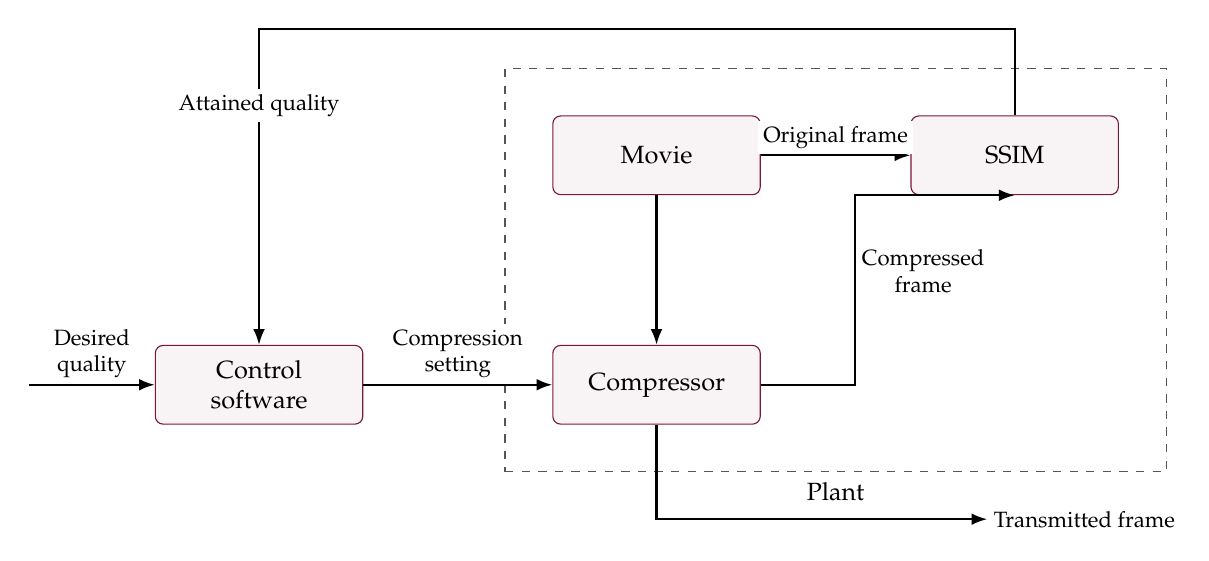
\begin{tikzpicture}[node distance=13mm and 17mm]
\node[process] (ctrl) {Control\\software};
\node[process,right=24mm of ctrl] (comp) {Compressor};
\node[process,above=19mm of comp] (movie) {Movie};
\node[process,right=19mm of movie] (ssim) {SSIM};
\draw[arr] (ctrl.west) ++(-16mm,0) -- node[lab,above]{Desired\\quality} (ctrl.west);
\draw[arr] (ctrl) -- node[lab,above]{Compression\\setting} (comp);
\draw[arr] (movie) -- (comp);
\draw[arr] (movie) -- node[lab,above]{Original frame} (ssim);
\draw[arr] (comp.east) -- ++(12mm,0) |- node[lab,pos=.3,right]{Compressed\\frame} (ssim.south);
\draw[arr] (ssim.north) -- ++(0,11mm) -| node[lab,pos=.65,above]{Attained quality} (ctrl.north);
\draw[arr] (comp.south) -- ++(0,-12mm) -- ++(42mm,0) node[lab,right]{Transmitted frame};
\begin{scope}[on background layer]\node[draw=muted,dashed,fit=(movie)(comp)(ssim),inner sep=6mm,label={[font=\small]below:Plant}] {};\end{scope}
\end{tikzpicture}
\caption{Detailed plant boundary from source p.\ 4. Both original and compressed frames reach SSIM; attained quality returns to the controller.}
\label{fig:compressor}
\end{figure}

The revised abstraction in source pp.\ 5--6 replaces these internals by a single plant block. The same reasoning can then be used for any reasonable plant within the modelling assumptions: learn the model online and adjust the control strategy. In the lecture's terminology, online control is a form of online planning. Combining learning with planning is the distinguishing feature of the intelligent system in this example.
\begin{figure}[htbp]\centering
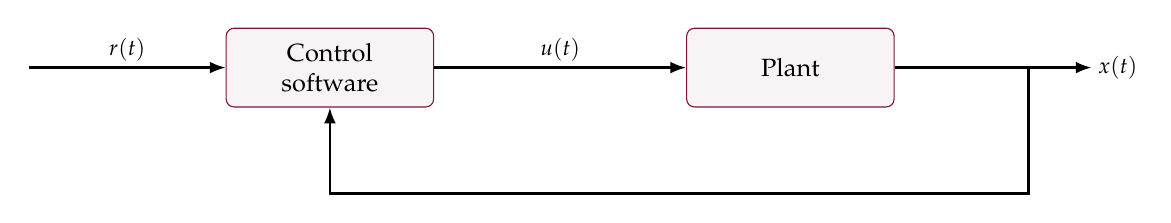
\begin{tikzpicture}
\node[process] (c) {Control\\software};
\node[process,right=32mm of c] (p) {Plant};
\draw[arr] (c.west) ++(-25mm,0) -- node[lab,above]{$r(t)$} (c.west);
\draw[arr] (c) -- node[lab,above]{$u(t)$} (p);
\draw[arr] (p.east) -- ++(25mm,0) coordinate (out) node[lab,right]{$x(t)$};
\draw[arr] ($(out)+(-8mm,0)$) -- ++(0,-16mm) -| (c.south);
\end{tikzpicture}
\caption{Abstract quality-feedback loop. The time-index convention is causal: $u(t)$ affects the next frame's quality $x(t+1)$.}
\label{fig:abstract}
\end{figure}
\FloatBarrier

\subsection{A simple plant model}
Let $x(t)$ denote the quality of the frame sent at discrete time $t$, and let $u(t)$ be the setting used for the next frame. The proposed model is
\begin{equation}\label{eq:plant}x(t+1)=\alpha u(t).\end{equation}
The scalar $\alpha$ is an unknown plant gain. The model has a one-step input-to-output delay and no explicit dependence on the previous quality. It is a deliberately simple local approximation, not a claim that all video content obeys a globally linear law.

The reference $r(t)$ specifies desired quality; for example $r(t)\equiv0.9$. The controller should make $x(t)$ close to $r(t)$. Choosing a model structure turns the broad task of learning a plant into the narrower task of estimating $\alpha$.

\clarify{The slides call $u$ a ``compression rate'', but do not specify the codec parameterization. With $\alpha>0$, increasing $u$ increases predicted quality. Thus $u$ must be interpreted as a setting with that orientation; it must not automatically be identified with a ratio for which larger values mean more destructive compression. The codec limits and feasible quality range are unspecified.}

\subsection{Online least-squares estimation}
At time $t$, use a sliding window of $w$ measured qualities
\[\widehat{x}(t),\widehat{x}(t-1),\ldots,\widehat{x}(t-w+1).\]
The corresponding model predictions are $\alpha u(t-1),\alpha u(t-2),\ldots,\alpha u(t-w)$. Each measurement must be paired with the input that produced it, one time step earlier.

Define the sum of squared errors
\begin{equation}\label{eq:sse}
J(\alpha)=\sum_{k=0}^{w-1}[\widehat{x}(t-k)-x(t-k)]^2
=\sum_{k=0}^{w-1}[\widehat{x}(t-k)-\alpha u(t-k-1)]^2.
\end{equation}
The slides call $J$ the Mean Squared Error (MSE); strictly the mean is $J/w$. Multiplication by the positive constant $1/w$ does not change the minimizing gain.

Differentiating with respect to $\alpha$ gives the complete sequence of steps used in the source:
\begin{align*}
\frac{dJ}{d\alpha}
&=\sum_{k=0}^{w-1}2[\widehat{x}(t-k)-\alpha u(t-k-1)][-u(t-k-1)]\\
&=2\sum_{k=0}^{w-1}[-\widehat{x}(t-k)u(t-k-1)+\alpha u^2(t-k-1)]\\
&=-2\sum_{k=0}^{w-1}\widehat{x}(t-k)u(t-k-1)
+2\alpha\sum_{k=0}^{w-1}u^2(t-k-1).
\end{align*}
Setting this derivative to zero yields
\begin{equation}\label{eq:estimate}
\widehat\alpha(t)=\frac{\displaystyle\sum_{k=0}^{w-1}\widehat{x}(t-k)u(t-k-1)}{\displaystyle\sum_{k=0}^{w-1}u^2(t-k-1)}.
\end{equation}
The source writes this estimate as $\alpha(t)$; a hat is added here to distinguish the estimate from the true plant gain. Every term uses known past inputs and observed qualities.

If $S_u=\sum_{k=0}^{w-1}u^2(t-k-1)>0$, then $d^2J/d\alpha^2=2S_u>0$, so the stationary point is the unique minimizer. If every input in the window is zero, $S_u=0$: the data do not identify $\alpha$, and the quotient is undefined. A usable implementation must handle this case and must not divide by a zero estimated gain when computing the controller.

\subsection{Integral control and its online realization}
The error is desired quality minus attained quality:
\begin{equation}\label{eq:error}e(t)=r(t)-x(t).\end{equation}
For a fixed gain $K>0$, the proposed law is
\begin{equation}\label{eq:integral}u(t)=K\sum_{k=0}^{t}e(k).\end{equation}
Persistent positive error increases the setting, while negative error decreases it. The slides refer to a PI (proportional-integral) controller. As written, \cref{eq:integral} is an integral-only law: there is no separate proportional term $K_Pe(t)$ in addition to the sum.

An accumulator avoids recomputing the full history:
\begin{align}\label{eq:controller}
z(t+1)&=z(t)+Ke(t),& z(0)&=0,\\
u(t)&=z(t)+Ke(t).\label{eq:controlleroutput}
\end{align}
Indeed, $z(t)=K\sum_{k=0}^{t-1}e(k)$ for fixed $K$, so the output equals \cref{eq:integral}. The current error is included immediately, and $u(t)=z(t+1)$. Therefore
\begin{align*}
u(t+1)&=z(t+1)+Ke(t+1)\\
&=z(t)+Ke(t)+Ke(t+1)=u(t)+Ke(t+1).
\end{align*}

\subsection{Closed-loop state equations and equilibrium}
Combining the plant, accumulator, and error gives
\begin{align*}
x(t+1)&=\alpha z(t)+\alpha Ke(t)
=\alpha[z(t)+K(r(t)-x(t))],\\
z(t+1)&=z(t)+Ke(t)=z(t)+K(r(t)-x(t)).
\end{align*}
Expanding the terms produces the two-dimensional system
\begin{align}
x(t+1)&=-\alpha Kx(t)+\alpha z(t)+\alpha Kr(t),\label{eq:closedx}\\
z(t+1)&=-Kx(t)+z(t)+Kr(t).\label{eq:closedz}
\end{align}
For $X(t)=[x(t),z(t)]^T$, the matrix form is
\begin{equation}\label{eq:closedmatrix}
X(t+1)=AX(t)+B_r r(t),\quad
A=\begin{bmatrix}-\alpha K&\alpha\\-K&1\end{bmatrix},\quad
B_r=\begin{bmatrix}\alpha K\\K\end{bmatrix}.
\end{equation}
Here the reference is the external input to the closed loop; it must not be confused with the compressor input $u$.

The design goals are (i) equilibrium tracking and (ii) asymptotic stability. For a constant reference $r^*$, equilibrium means $x(t+1)=x(t)=x^*$ and $z(t+1)=z(t)=z^*$. From the second equation, $K(r^*-x^*)=0$, so $K\ne0$ implies $x^*=r^*$. Substitution gives exactly the source's equilibrium equations:
\begin{align*}
r^*&=-\alpha Kr^*+\alpha z^*+\alpha Kr^*,\\
z^*&=-Kr^*+z^*+Kr^*.
\end{align*}
They reduce to $r^*=\alpha z^*$ and the identity $z^*=z^*$; hence
\begin{equation}\label{eq:eqpoint}x^*=r^*,\qquad z^*=\frac{r^*}{\alpha},\qquad u^*=\frac{r^*}{\alpha}.\end{equation}
This requires $\alpha\ne0$ and a feasible actuator setting. The equilibrium location does not depend on $K$, but convergence to it does. A constant-reference equilibrium does not establish exact tracking of arbitrary time-varying references.

\subsection{Stability and corrected pole placement}\label{sec:poles}
For a discrete-time linear system, all eigenvalues of $A$ must have modulus strictly less than one for asymptotic stability. Direct expansion gives
\begin{align}
\det(\lambda I-A)
&=\det\begin{bmatrix}\lambda+\alpha K&-\alpha\\K&\lambda-1\end{bmatrix}\nonumber\\
&=(\lambda+\alpha K)(\lambda-1)+\alpha K\nonumber\\
&=\lambda^2+(\alpha K-1)\lambda
=\lambda[\lambda-(1-\alpha K)].\label{eq:charpoly}
\end{align}
Thus the two eigenvalues are
\begin{equation}\label{eq:poles}\lambda_1=0,\qquad\lambda_2=1-\alpha K.\end{equation}
The constant terms cancel; equivalently $\det A=0$. Therefore
\begin{equation}\label{eq:gaincondition}|1-\alpha K|<1\quad\Longleftrightarrow\quad0<\alpha K<2.\end{equation}
For the intended $K>0$, this requires a positive plant gain and $0<K<2/\alpha$.

\begin{concept}{Correct gain for a chosen nonzero pole}
For a known positive $\alpha$, choose $p\in(0,1)$ and set
\[K=\frac{1-p}{\alpha}.\]
The closed-loop eigenvalues are then $0$ and $p$. This is the final gain formula in the slides, but its correct justification is \cref{eq:charpoly}, not the intermediate two-pole argument in source pp.\ 20--24.
\end{concept}

Substitution yields the source's final expanded and error-based forms:
\begin{align}
x(t+1)&=-(1-p)x(t)+\alpha z(t)+(1-p)r(t),\\
z(t+1)&=-\frac{1-p}{\alpha}x(t)+z(t)+\frac{1-p}{\alpha}r(t),\\
x(t+1)&=\alpha z(t)+(1-p)e(t),\\
z(t+1)&=z(t)+\frac{1-p}{\alpha}e(t).
\end{align}
For a constant reference and a consistent plant history, $x(t)=\alpha z(t)$ after the first plant step. Consequently $x(t+1)=p x(t)+(1-p)r^*$, and the tracking error contracts by $p$. Smaller positive $p$ gives faster nominal convergence; implementation constraints and model error are not captured by this observation.

\subsection{Accounting for the source's intermediate derivation}\label{sec:sourcepoles}
\begin{sourcecorrection}{characteristic polynomial on source p.\ 20}
The source first gives the correct determinant expression, but expands it as
\[\lambda^2+(\alpha K-1)\lambda+\alpha K=0.\]
For the stated matrix $A$, the constant terms cancel. The correct characteristic polynomial is
\[\lambda^2+(\alpha K-1)\lambda=\lambda\bigl[\lambda-(1-\alpha K)\bigr],\]
so the poles are $0$ and $1-\alpha K$.
\end{sourcecorrection}
Pages 21--23 use the source polynomial to propose poles $p_1,p_2$. Reconstructing that argument with the missing factor of $\lambda$ in the source's factor expansion restored gives
\begin{align*}
(\lambda-p_1)(\lambda-p_2)&=\lambda^2-(p_1+p_2)\lambda+p_1p_2,\\
1-\alpha K&=p_1+p_2,\qquad \alpha K=p_1p_2,\\
1-p_1p_2&=p_1+p_2,\\
1-p_1&=p_2(1+p_1),\qquad p_2=\frac{1-p_1}{1+p_1},\\
K&=\frac{p_1p_2}{\alpha}=\frac{p_1}{\alpha}\frac{1-p_1}{1+p_1}.
\end{align*}
These coefficient relations concern the erroneous polynomial, not the actual closed-loop matrix. For the actual matrix, coefficient matching instead gives $p_1+p_2=1-\alpha K$ and $p_1p_2=0$: both poles cannot be freely assigned away from zero.

Page 24 also argues from $p_1(1-p_1)/(1+p_1)\in(0,1)$ to an arbitrary substitution $1-p$ with $p\in(0,1)$. Membership in an interval does not establish that the expression attains every value in that interval. In fact its maximum on $(0,1)$ is $3-2\sqrt2$, reached at $p_1=\sqrt2-1$. The final formula $K=(1-p)/\alpha$ is nevertheless valid by the independent corrected calculation above.

The intended design insight is retained: adjusting $K$ inversely with the plant gain keeps the \emph{nominal} poles fixed. If an estimate differs from the true gain, that cancellation is only approximate.

\subsection{Adaptive operation and initialization}
The source's summary combines learning with control. In notation that distinguishes estimate from truth, its update is
\begin{align}
\widehat\alpha(t)&=\frac{\sum_{k=0}^{w-1}\widehat{x}(t-k)u(t-k-1)}{\sum_{k=0}^{w-1}u^2(t-k-1)},\label{eq:adaptiveestimate}\\
K(t)&=\frac{1-p}{\widehat\alpha(t)},\quad 0<p<1,\\
\widetilde{x}(t+1)&=\widehat\alpha(t)u(t),\label{eq:prediction}\\
z(t+1)&=z(t)+K(t)[r(t)-x(t)],\\
u(t)&=z(t)+K(t)[r(t)-x(t)].\label{eq:adaptiveu}
\end{align}
The tilde marks a model prediction: actual measured quality need not equal it. The estimator uses $\widehat{x}$ for measurements in the source; the feedback equations use $x$ for attained quality. In practice the feedback signal is the available measurement.

The summary states $z(0)=0$, $x(0)=\cdots=x(w-1)=1$, and control starting at $t=w$. This describes an initial full-quality phase, but does not specify its input settings, the measurement $x(w)$, or how the accumulator is handled before control begins. Those are implementation details that must be supplied; measured values must not be fabricated. At $t=w$, the displayed estimator needs the pairs $(\widehat{x}(1),u(0)),\ldots,(\widehat{x}(w),u(w-1))$.

With variable gains the accumulator contains a weighted sum of past errors. In general it is not $K(t)\sum e(k)$, because each error was accumulated with the gain used at its own time.

For a fixed true gain $\alpha$ and a frozen estimate $\widehat\alpha$, the actual nonzero pole is
\[1-\alpha\frac{1-p}{\widehat\alpha},\]
so nominal pole placement alone does not prove stability under estimation error. Nor does checking every frozen matrix establish stability of an arbitrary time-varying adaptive system. Actuator limits, noise, changes in movie content, and estimation safeguards require further analysis not present in these slides.

\begin{figure}[htbp]\centering
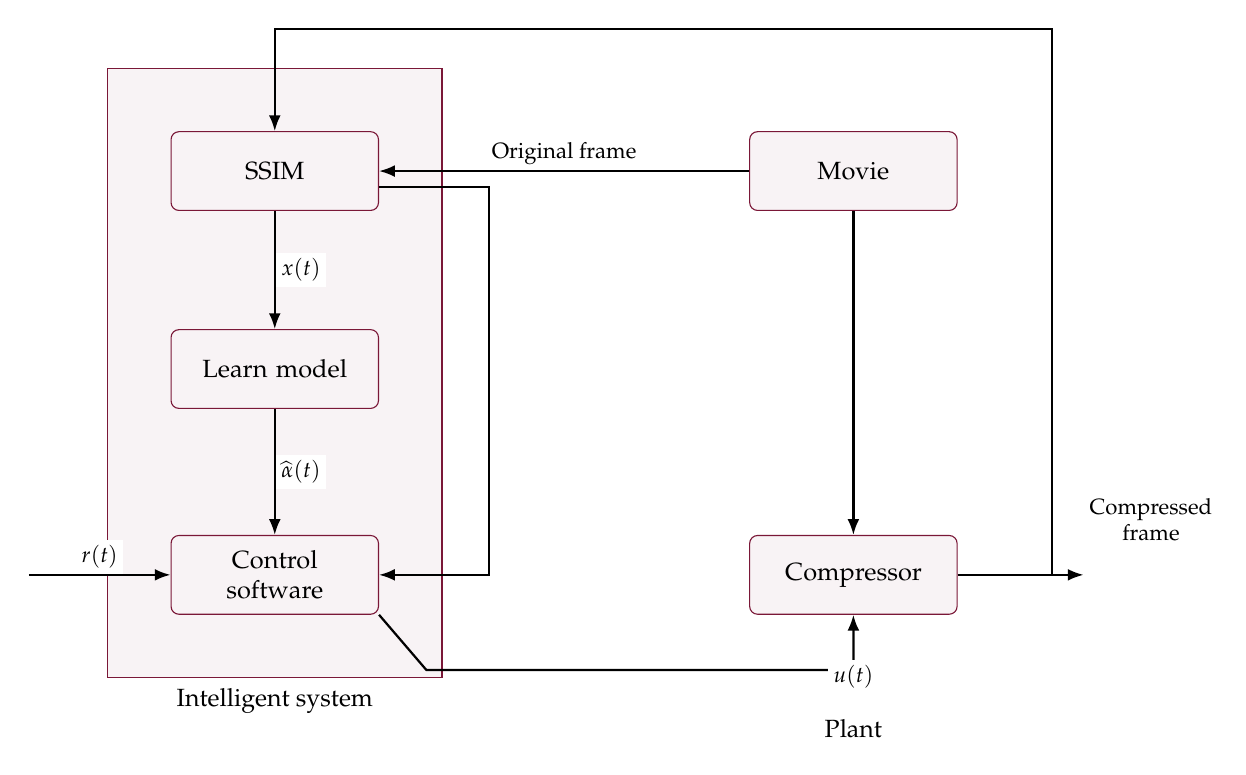
\begin{tikzpicture}
\node[process] (ssim) {SSIM};
\node[process,below=15mm of ssim] (learn) {Learn model};
\node[process,below=16mm of learn] (ctrl) {Control\\software};
\node[process,right=47mm of ssim] (movie) {Movie};
\node[process,right=47mm of ctrl] (comp) {Compressor};
\draw[arr] (movie.west) -- node[lab,above]{Original frame} (ssim.east);
\draw[arr] (movie) -- (comp);
\draw[arr] (ssim.south) -- node[lab,right]{$x(t)$} (learn.north);
\draw[arr] (learn) -- node[lab,right]{$\widehat\alpha(t)$} (ctrl);
\draw[arr] (ssim.east) ++(0,-2mm) -- ++(14mm,0) |- (ctrl.east);
\draw[arr] (ctrl.west) ++(-18mm,0) -- node[lab,above]{$r(t)$} (ctrl.west);
\draw[arr] (ctrl.south east) -- ++(6mm,-7mm) -| node[lab,pos=.6,below]{$u(t)$} (comp.south);
\draw[arr] (comp.east) -- ++(16mm,0) coordinate (out);
\draw[arr] ($(out)+(-4mm,0)$) |- ($(ssim.north)+(0,13mm)$) -- (ssim.north);
\node[lab,right] at ($(comp.east)+(16mm,7mm)$) {Compressed\\frame};
\begin{scope}[on background layer]\node[draw=wine,fill=pale,fit=(ssim)(learn)(ctrl),inner sep=8mm,label={[font=\small]below:Intelligent system}] {};\end{scope}
\node[font=\small,below=12mm of comp] {Plant};
\end{tikzpicture}
\caption{Revised boundary in source p.\ 27: SSIM, model learning, and control belong to the intelligent system; movie and compressor form the plant. Past settings $u$ are also required by the estimator, although that connection is omitted in the source diagram.}
\label{fig:adaptive}
\end{figure}\FloatBarrier
\subsection{Key takeaways}
The case study combines online parameter estimation, integral feedback, and nominal pole placement. Preserve the one-frame delay in every data pair. The least-squares denominator must be nonzero, the gain used in a division must be valid, and the requested equilibrium must be feasible. For the stated fixed-gain model, the poles are $0$ and $1-\alpha K$; with exact model knowledge, $K=(1-p)/\alpha$ places the nonzero pole at $p$.

\module{Continuous-time dynamical systems}{2000-ct-systems.pdf, pp.\ 1--6; September 27, 2026}
The source module is titled \emph{Introduction to Continuous-Time Dynamical Systems}, with subtitle \emph{Fundamentals, State-Space Representation, and Robotics Applications}.

\subsection{State-space representation}
Continuous-time models describe physical processes at times $t\in\R_{\ge0}$. Their general nonlinear form is
\begin{equation}\label{eq:ctgeneral}
\dot x(t)=\frac{dx(t)}{dt}=f(t,x(t),u(t)),\qquad y(t)=h(t,x(t),u(t)).
\end{equation}
The state $x(t)\in\R^n$ records the variables needed, together with future inputs, to determine future behaviour. In physical examples, these encode memory and stored energy. The input $u(t)\in\R^m$ represents controls, forces, or disturbances; $y(t)$ is the output. The slides call the state a minimum set of variables. Minimality avoids redundancy, but a valid state representation need not be minimal.

\begin{concept}{Linear time-invariant special case}
A Linear Time-Invariant (LTI) model has constant matrices:
\[\dot x=Ax+Bu,\qquad y=Cx+Du.\]
Here $A\in\R^{n\times n}$ is the state matrix and $B\in\R^{n\times m}$ the input matrix. For $y\in\R^q$, the dimensions are $C\in\R^{q\times n}$ and $D\in\R^{q\times m}$. The term $Du$ is direct input-to-output dependence.
\end{concept}

\subsection{Quadrotor: Newton--Euler dynamics}
A quadrotor has six physical Degrees of Freedom (DOFs), three translational and three rotational. Including rates gives twelve state components:
\[x=[\mathbf p^T,\mathbf v^T,\Theta^T,\boldsymbol\omega^T]^T\in\R^{12}.\]
Position is $\mathbf p=[x,y,z]^T$, velocity is $\mathbf v=[\dot x,\dot y,\dot z]^T$, Euler angles are $\Theta=[\phi,\theta,\psi]^T$, and body angular velocity is $\boldsymbol\omega=[p,q,r]^T$. The position vector $\mathbf p$ is distinct from the scalar angular-rate component $p$.

The four inputs are collective thrust $F_T$ and torques $\boldsymbol\tau=[\tau_x,\tau_y,\tau_z]^T$. The source equations are
\begin{align}
\dot{\mathbf p}&=\mathbf v,\\
\dot{\mathbf v}&=-g\mathbf e_3+\frac1m R(\Theta)\begin{bmatrix}0\\0\\F_T\end{bmatrix},\label{eq:quadtrans}\\
\dot\Theta&=W(\Theta)\boldsymbol\omega,\\
I\dot{\boldsymbol\omega}&=\boldsymbol\tau-\boldsymbol\omega\times(I\boldsymbol\omega).\label{eq:quadrot}
\end{align}
Here $g$ is gravitational acceleration, $m$ is mass, $\mathbf e_3=[0,0,1]^T$, $R$ rotates body thrust into inertial coordinates, $W$ converts body angular velocity into Euler-angle rates, and $I$ is the inertia matrix. The cross product represents gyroscopic coupling. The gravity sign follows the source's vertical-axis convention.

The model is nonlinear and coupled: changing orientation changes thrust direction. Four inputs control six configuration DOFs, so the system is underactuated. The source does not specify the Euler-angle convention or the explicit matrix $W$; these must be fixed before implementation.

\subsection{Robotic arm: Euler--Lagrange dynamics}
An $n$-joint manipulator has joint positions $q\in\R^n$, joint velocities $\dot q$, state $x=[q^T,\dot q^T]^T\in\R^{2n}$, and torque input $u=\tau\in\R^n$. Its dynamics are
\begin{equation}\label{eq:arm}M(q)\ddot q+C(q,\dot q)\dot q+g(q)=\tau.\end{equation}
The configuration-dependent inertia is $M(q)$, the Coriolis/centripetal term is $C(q,\dot q)\dot q$, and the gravitational torque is $g(q)$. This vector-valued $g(q)$ differs from the quadrotor's scalar gravity constant.

Solving for acceleration converts the second-order model to first-order state space:
\begin{equation}
\frac{d}{dt}\begin{bmatrix}q\\\dot q\end{bmatrix}
=\begin{bmatrix}\dot q\\M(q)^{-1}\bigl(\tau-C(q,\dot q)\dot q-g(q)\bigr)\end{bmatrix}.
\end{equation}
In standard independent-joint rigid-body coordinates, the inertia matrix is positive definite and invertible. First-order conversion exposes the state but does not remove nonlinear coupling.

\subsection{Equilibrium, stability, and controllability}
An equilibrium $x_e$ under constant input $u_e$ satisfies $f(t,x_e,u_e)=0$. If $f$ is explicitly time-dependent, the equality must hold at every relevant time.

\begin{concept}{Lyapunov stability}
An equilibrium is stable if starting sufficiently close makes the trajectory remain arbitrarily close for all future time. For every $\varepsilon>0$, there is a $\delta>0$ such that
\[\|x(t_0)-x_e\|<\delta\ \Longrightarrow\ \|x(t)-x_e\|<\varepsilon\quad(t\ge t_0).\]
Asymptotic stability additionally requires convergence $x(t)\to x_e$ for nearby initial states. The slide's phrase ``remain bounded'' is too weak: staying in a large bounded region need not mean staying close.
\end{concept}
For an autonomous LTI system $\dot x=Ax$, the origin is asymptotically stable precisely when
\begin{equation}\label{eq:ctstable}\operatorname{Re}\lambda_i(A)<0\qquad(i=1,\ldots,n).\end{equation}
Eigenvalues on the imaginary axis do not meet this strict condition and require separate analysis for marginal stability.

\emph{Controllability} is the ability to steer $x(t_0)$ to a target $x(t_f)$ using admissible inputs. The slides say bounded inputs. Inputs bounded on a finite interval must be distinguished from a prescribed actuator-amplitude bound: a fixed bound can restrict finite-time reachability even for a controllable LTI pair.

\Needspace{8\baselineskip}
\subsection{Taxonomy of continuous physical systems}
The source comparison is split into two readable tables. Dimensions refer to the chosen models, not to every possible model of each device.
\begin{table}[htbp]\centering\small
\caption{States and inputs in the continuous-time taxonomy.}
\begin{tabularx}{\textwidth}{@{}P{27mm}YY@{}}\toprule
System & State & Input\\\midrule
Quadrotor & Position, attitude, rates ($n=12$). & Motor thrusts / torques ($m=4$).\\\addlinespace
Robotic arm & Joint angles and rates ($n=2k$ for $k$ joints). & Joint torques ($m=k$).\\\addlinespace
Self-driving car & Coordinates, yaw, speed; source reports $n=5$. & Steering and acceleration ($m=2$).\\\addlinespace
Inverted pendulum & Cart position, angle, and rates ($n=4$). & Cart force ($m=1$).\\\bottomrule
\end{tabularx}\end{table}
\begin{table}[htbp]\centering\small
\caption{Actuation and dynamic features in the continuous-time taxonomy.}
\begin{tabularx}{\textwidth}{@{}P{27mm}P{29mm}Y@{}}\toprule
System & Classification & Features\\\midrule
Quadrotor & Underactuated & Aerodynamic / gyroscopic coupling.\\\addlinespace
Robotic arm & Fully actuated & Nonlinear inertia and Coriolis forces.\\\addlinespace
Self-driving car & Non-holonomic & Kinematic constraints and dynamic tire slip.\\\addlinespace
Inverted pendulum & Underactuated & Unstable upright (zenith) equilibrium.\\\bottomrule
\end{tabularx}\end{table}\FloatBarrier
\clarify{The car row states $n=5$ without listing all five components; no missing component is invented here. Non-holonomic describes a motion constraint, not an input count. Aerodynamic effects are listed in the taxonomy but no explicit drag term appears in the displayed quadrotor model.}

\subsection{Key takeaways}
Continuous dynamics specify rates of change. Equilibrium, stability, and controllability ask where motion can stop, how perturbations evolve, and what states inputs can reach. They are distinct properties.

\module{Discrete-time dynamical systems}{3000-dt-systems.pdf, pp.\ 1--14; September 27, 2026}
The module is titled \emph{Introduction to Discrete-Time Dynamical Systems}, with subtitle \emph{State-Space Models, Discretization \& Student Walkthroughs}. It connects physical dynamics with digital execution and naturally discrete models.

\subsection{Difference equations and digital execution}
For $k\in\mathbb N_0=\{0,1,2,\ldots\}$, the general state and output equations are
\begin{equation}x_{k+1}=f(k,x_k,u_k),\qquad y_k=h(k,x_k,u_k).\end{equation}
The LTI form is
\begin{equation}\label{eq:dtlti}x_{k+1}=Ax_k+Bu_k,\qquad y_k=Cx_k+Du_k.\end{equation}
Here $x_k\in\R^n$, $u_k\in\R^m$, $A\in\R^{n\times n}$, and $B\in\R^{n\times m}$. A difference equation specifies the next state rather than its instantaneous derivative.

Physical systems evolve continuously, but microcontrollers update at sampling times $t_k=kT_s$, with sampling period $T_s>0$. Discretization converts, for example, $\dot x=A_cx$ into $x_{k+1}=A_dx_k$. Its accuracy depends on how $A_d$ is obtained.

Knowing the initial state and input sequence gives the recursive predictions
\begin{align*}
x_1&=Ax_0+Bu_0,\\
x_2&=Ax_1+Bu_1=A^2x_0+ABu_0+Bu_1.
\end{align*}
The second equation shows how an earlier action continues to affect future states through the transition matrix.

\subsection{Digital motor control: forward Euler}
A direct-current (DC) motor is modelled using angle $\theta$, angular velocity $\omega$, and voltage input $u$:
\begin{equation}\label{eq:motorct}\dot\theta=\omega,\qquad\dot\omega=-\alpha\omega+\beta u.\end{equation}
Here $\alpha$ is a damping coefficient and $\beta$ converts voltage into an acceleration contribution. These are motor parameters, unrelated to the compressor's gain.

Forward Euler approximates $\dot x(t_k)$ by $(x_{k+1}-x_k)/T_s$. Applying this to both equations gives
\begin{align*}
\frac{\theta_{k+1}-\theta_k}{T_s}&=\omega_k
&&\Longrightarrow\ \theta_{k+1}=\theta_k+T_s\omega_k,\\
\frac{\omega_{k+1}-\omega_k}{T_s}&=-\alpha\omega_k+\beta u_k
&&\Longrightarrow\ \omega_{k+1}=(1-\alpha T_s)\omega_k+\beta T_su_k.
\end{align*}
Thus the Euler matrices are
\begin{equation}\label{eq:eulermotor}
\begin{bmatrix}\theta_{k+1}\\\omega_{k+1}\end{bmatrix}
=\underbrace{\begin{bmatrix}1&T_s\\0&1-\alpha T_s\end{bmatrix}}_{A_{\mathrm E}}
\begin{bmatrix}\theta_k\\\omega_k\end{bmatrix}
+\underbrace{\begin{bmatrix}0\\\beta T_s\end{bmatrix}}_{B_{\mathrm E}}u_k.
\end{equation}
Voltage $u_k$ first changes $\omega_{k+1}$ and only affects angle at step $k+2$ in this approximation, because the angle update evaluates velocity at the start of the interval.

\subsection{Exact integration under zero-order hold}
A Zero-Order Hold (ZOH) keeps $u$ constant during each sample interval. Let $\tau\in[0,T_s]$ be local time from $t_k$, so $u(t_k+\tau)=u_k$. For $\alpha\ne0$, solving the velocity equation gives
\begin{equation}\label{eq:motoromega}
\omega(t_k+\tau)=\omega_ke^{-\alpha\tau}+\frac{\beta u_k}{\alpha}(1-e^{-\alpha\tau}).
\end{equation}
Integrating velocity gives the source's two contributions to displacement:
\begin{align}
\theta_{k+1}&=\theta_k+\underbrace{\int_0^{T_s}\omega_ke^{-\alpha\tau}\,d\tau}_{I_1}
+\underbrace{\int_0^{T_s}\frac{\beta u_k}{\alpha}(1-e^{-\alpha\tau})\,d\tau}_{I_2},\\
I_1&=\frac{1-e^{-\alpha T_s}}\alpha\omega_k,\\
I_2&=\frac\beta\alpha\left(T_s-\frac{1-e^{-\alpha T_s}}\alpha\right)u_k.
\end{align}
These integrals and the velocity at $\tau=T_s$ imply the exact ZOH matrices
\begin{equation}\label{eq:zohmotor}
A_{\mathrm Z}=\begin{bmatrix}1&\dfrac{1-e^{-\alpha T_s}}\alpha\\[2mm]0&e^{-\alpha T_s}\end{bmatrix},\quad
B_{\mathrm Z}=\begin{bmatrix}\dfrac\beta\alpha\left(T_s-\dfrac{1-e^{-\alpha T_s}}\alpha\right)\\[2mm]\dfrac\beta\alpha(1-e^{-\alpha T_s})\end{bmatrix}.
\end{equation}
The full matrices are an explanatory derivation from the source's integrals. In general, for LTI dynamics under ZOH,
\[A_d=e^{A_cT_s},\qquad B_d=\int_0^{T_s}e^{A_c\tau}B_c\,d\tau.\]

\subsection{Exact and approximate displacement}
Expanding the exponential gives
\[e^{-\alpha T_s}=1-\alpha T_s+\tfrac12\alpha^2T_s^2+O(T_s^3).\]
The source uses $I_1\approx T_s\omega_k$ and $I_2\approx\tfrac12\beta T_s^2u_k$ to emphasize the direct within-interval input effect:
\[\theta_{k+1}\approx\theta_k+T_s\omega_k+\tfrac12\beta T_s^2u_k.\]
This mixes the first-order velocity term with the leading input term. A consistent second-order approximation must also retain damping:
\begin{equation}\label{eq:motortaylor}
\theta_{k+1}=\theta_k+T_s\omega_k+\tfrac12(-\alpha\omega_k+\beta u_k)T_s^2+O(T_s^3).
\end{equation}
Likewise the slide comparison
\[B_{\mathrm E}=\begin{bmatrix}0\\\beta T_s\end{bmatrix},\qquad
B_{\mathrm Z}\approx\begin{bmatrix}\frac12\beta T_s^2\\\beta T_s\end{bmatrix}\]
keeps the leading nonzero term in each component; it is not the exact input matrix. The second-order lower component is $\beta T_s-\tfrac12\alpha\beta T_s^2$.

\begin{sourcecorrection}{ZOH does not imply constant total acceleration}
ZOH holds $u_k$ constant, not $\dot\omega=-\alpha\omega+\beta u_k$. For nonzero damping, velocity changes and therefore acceleration changes during the interval. The term $\tfrac12\beta u_kT_s^2$ is the leading input displacement. For $\alpha=0$ it is exact, with
\[A_d=\begin{bmatrix}1&T_s\\0&1\end{bmatrix},\qquad B_d=\begin{bmatrix}\frac12\beta T_s^2\\\beta T_s\end{bmatrix}.\]
\end{sourcecorrection}

\subsection{Leslie population dynamics}
The Leslie model tracks female population counts in $m$ age cohorts across breeding seasons. Its state is $x_k=[n_{1,k},\ldots,n_{m,k}]^T$, with $n_{i,k}$ the population in age class $i$. In the three-class example,
\begin{equation}\label{eq:leslie}
\begin{bmatrix}n_{1,k+1}\\n_{2,k+1}\\n_{3,k+1}\end{bmatrix}
=\underbrace{\begin{bmatrix}f_1&f_2&f_3\\s_1&0&0\\0&s_2&0\end{bmatrix}}_{L}
\begin{bmatrix}n_{1,k}\\n_{2,k}\\n_{3,k}\end{bmatrix}.
\end{equation}
Fecundity $f_i\ge0$ is the average female offspring per member of class $i$. The source assumes $s_i\in(0,1]$, the survival probability from class $i$ to $i+1$. The first row counts newborns:
\[n_{1,k+1}=f_1n_{1,k}+f_2n_{2,k}+f_3n_{3,k}.\]
The subdiagonal describes aging: $n_{2,k+1}=s_1n_{1,k}$ and $n_{3,k+1}=s_2n_{2,k}$.

The source uses the dominant eigenvalue as the long-term growth factor: $\lambda_1>1$ indicates expansion, $\lambda_1<1$ decline toward extinction, and $\lambda_1=1$ a stationary growth factor.

\begin{supplementary}{Conditions for asymptotic age-profile convergence}
Under the standard condition that $L$ is primitive and the initial population is nonzero and nonnegative, $x_k$ approaches the form $c\lambda_1^kv_1$, with positive dominant eigenvector $v_1$ and $c>0$. Normalized age proportions approach the profile of $v_1$. Suitable irreducibility and aperiodicity assumptions are needed for this convergence; without them, cyclic counterexamples are possible.
\end{supplementary}

\subsection{PageRank as a Markov chain}
PageRank models a random surfer moving across $N$ webpages. The column vector $p_k\in\R^N$ contains probabilities $p_{i,k}\ge0$ with $\sum_i p_{i,k}=1$. The source defines a row-stochastic matrix by
\[M_{ij}=\mathbb P(\text{page }j\text{ at }k+1\mid\text{page }i\text{ at }k),\quad\sum_jM_{ij}=1.\]
Consequently,
\begin{equation}p_{k+1}^T=p_k^TM\quad\Longleftrightarrow\quad p_{k+1}=M^Tp_k.\end{equation}
The transpose matters: rows describe outgoing transitions, whereas $p_k$ is a column.

The damping adjustment is
\begin{equation}\label{eq:google}\overline M=dM+\frac{1-d}{N}\mathbf1_{N\times N},\qquad d=0.85,\end{equation}
where $\mathbf1$ is the all-ones matrix. The surfer follows links with probability $0.85$ and teleports uniformly with probability $0.15$.

\begin{supplementary}{Dangling pages in PageRank}
A page with no outgoing links must first receive a valid stochastic row, conventionally a uniform row. A zero row would otherwise give row sum $1-d$, not 1, after the adjustment. Teleportation also prevents trapping in closed groups of pages and removes periodicity.
\end{supplementary}

For stochastic $M$ and $0<d<1$, the adjusted matrix is strictly positive. Power iteration converges to a unique stationary distribution:
\begin{equation}p_{k+1}=\overline M^Tp_k,\qquad p^*=\overline M^Tp^*.\end{equation}
The stationary eigenvalue is $1$. Convergence occurs within the probability simplex, not toward zero in the full vector space, since total probability remains one.

\subsection{Discrete susceptible--infectious--recovered dynamics}
The Susceptible--Infectious--Recovered (SIR) model uses susceptible $S_k$, infectious $I_k$, and recovered $R_k$ populations at day $k$:
\begin{align}
S_{k+1}&=S_k-\beta S_kI_k,\\
I_{k+1}&=I_k+\beta S_kI_k-\gamma I_k,\\
R_{k+1}&=R_k+\gamma I_k.
\end{align}
New infections are $\beta S_kI_k$; recoveries are $\gamma I_k$. The slides call $\beta$ a daily infection parameter per contact and $\gamma$ a daily recovery parameter. Units of $\beta$ depend on whether compartments are counts or fractions: no explicit division by population size occurs in these equations. Their sum conserves $S_k+I_k+R_k$.

For $I_k>0$, infection grows in a step if and only if $\beta S_k>\gamma$. With $\gamma>0$, the source defines the initial reproduction quantity
\begin{equation}\mathcal R_0=\frac{\beta S_0}{\gamma}.\end{equation}
Thus $\mathcal R_0>1$ gives initial growth. Subsequent growth depends on $S_k$; the threshold does not imply indefinite increase. Nonnegative compartments also require admissible step parameters. For example, $0\le\gamma\le1$ and $0\le\beta I_k\le1$ prevent transfers exceeding the available compartments.

\subsection{Schur stability and exact sampling}
For the autonomous LTI recurrence $x_{k+1}=Ax_k$, the origin is asymptotically stable exactly when
\begin{equation}\label{eq:schur}|\lambda_i(A)|<1\qquad(i=1,\ldots,n).\end{equation}
Such $A$ is \emph{Schur stable}. In continuous time the criterion is negative real part; in discrete time it is membership in the open unit disk.

For exact sampling, $A_d=e^{A_cT_s}$ maps a continuous eigenvalue $s$ to
\begin{equation}z=e^{sT_s},\qquad |z|=e^{\operatorname{Re}(s)T_s}.\end{equation}
For $T_s>0$, the left half-plane maps into the unit disk. Euler instead maps $s$ to $1+sT_s$, and can lose stability for an excessive step size.

\subsection{Discrete Lyapunov analysis}
The matrix $A$ is Schur stable if and only if for every symmetric $Q\succ0$ there exists a unique symmetric $P\succ0$ satisfying
\begin{equation}\label{eq:lyapunov}A^TPA-P=-Q.\end{equation}
For $V(x_k)=x_k^TPx_k$ and $x_k\ne0$,
\begin{align}
\Delta V(x_k)&=V(x_{k+1})-V(x_k)\nonumber\\
&=x_k^T(A^TPA-P)x_k=-x_k^TQx_k<0.
\end{align}
Positive definiteness relates $V$ to state magnitude, so the decreasing quadratic energy establishes convergence to zero. At the origin, $V=0$ and $\Delta V=0$; the strict inequalities in the source implicitly exclude that point.

\subsection{Comparative taxonomy}
\begin{table}[htbp]\centering\small
\caption{Discrete models and possible controls listed in the source.}
\begin{tabularx}{\textwidth}{@{}P{24mm}YY@{}}\toprule
Domain & State and evolution & Input / control listed\\\midrule
Digital control & Position and speed ($n=2$); ZOH $A_d=e^{A_cT_s}$. & Motor voltage ($m=1$).\\\addlinespace
Leslie ecology & Cohort counts ($n=m$); nonnegative $L$. & Culling / harvesting.\\\addlinespace
PageRank DTMC & Page probabilities ($n=N$); stochastic $\overline M^T$. & Damping / teleportation $d$.\\\addlinespace
Discrete SIR & Susceptible, infectious, recovered ($n=3$); nonlinear recurrence. & Vaccination factor.\\\bottomrule
\end{tabularx}\end{table}
DTMC means Discrete-Time Markov Chain. In the Leslie row, $m$ denotes cohorts rather than input dimension. Harvesting and vaccination are mentioned as possible interventions, but no such terms appear in the preceding equations.

The source lists $|\lambda(A_d)|<1$ for digital control, $\lambda_1\gtrless1$ for Leslie growth, $\lambda_1=1$ for PageRank convergence, and $\mathcal R_0<1$ for declining infection. These address different properties. In particular, the open-loop motor's angle integrator gives an eigenvalue $1$: the full open-loop state is not asymptotically stable at zero. PageRank convergence needs its stochastic assumptions, while the SIR threshold concerns infection rather than global asymptotic stability of all compartments.
\FloatBarrier
\subsection{Key takeaways}
Discrete models can describe sampled physics or naturally staged processes. Preserve input timing, matrix transposes, and units. Distinguish exact discretization from numerical approximation, and distinguish LTI stability from the growth and convergence properties of other models.

\module{Optimal control in continuous time}{1000-opt-ctr-ct-sys.pdf, pp.\ 1--6; September 27, 2026}
The module subtitle is \emph{Formulation, Pontryagin's Minimum Principle, and HJB Equations}. Modelling specifies how a system evolves; optimal control chooses admissible actions to minimize a stated performance index.

\subsection{Problem formulation}
Choose a control trajectory $u^*(t)$ over $[t_0,t_f]$ to minimize
\begin{equation}\label{eq:ctcost}
J(u)=\phi(x(t_f),t_f)+\int_{t_0}^{t_f}L(t,x(t),u(t))\,dt
\end{equation}
subject to
\[\dot x(t)=f(t,x(t),u(t)),\quad x(t_0)=x_0,\quad u(t)\in\Omega\subseteq\R^m,\quad x(t_f)\in S_f\subseteq\R^n.\]
The state is $x\in\R^n$. The function $L$ is the running cost (also called the Lagrangian), and $\phi$ is the terminal cost. The source distinguishes the set $\mathcal U$ of admissible input trajectories from the pointwise input set $\Omega$. The final time may be fixed or free in the general formulation.

The terminal set encodes a required destination; the terminal cost expresses a preference among final states. These have different roles. Subsequent simple boundary formulas assume a free terminal state unless indicated otherwise. The finite-horizon HJB and LQR formulas below use a fixed $t_f$.

\subsection{Pontryagin's minimum principle}
The \emph{Hamiltonian} combines running cost with the effect of state motion:
\begin{equation}\label{eq:hamiltonian}
H(t,x,u,\lambda)=L(t,x,u)+\lambda^Tf(t,x,u).
\end{equation}
It maps $[t_0,t_f]\times\R^n\times\R^m\times\R^n$ to $\R$. The vector $\lambda(t)\in\R^n$ is a costate (adjoint), not an eigenvalue. Along an optimal trajectory, it describes the sensitivity associated with the dynamic constraints.

In the normal smooth setting used by the slides, Pontryagin's Minimum Principle (PMP) gives the following necessary conditions, evaluated along $(x^*,u^*,\lambda^*)$:
\begin{align}
\dot x^*(t)&=\nabla_\lambda H=f(t,x^*(t),u^*(t)),\\
\dot\lambda^*(t)&=-\nabla_xH
=-\nabla_xL-\left(\frac{\partial f}{\partial x}\right)^T\lambda^*(t),\label{eq:ctcostate}\\
u^*(t)&\in\argmin_{u\in\Omega}H(t,x^*(t),u,\lambda^*(t)),\label{eq:pmpmin}\\
\lambda^*(t_f)&=\nabla_x\phi(x^*(t_f),t_f)\quad\text{if the terminal state is free}.\label{eq:transversality}
\end{align}
\formulanote{$x$ is the state, $u$ the control, $L$ the running cost, $\phi$ the terminal cost, $\lambda$ the costate, and $\Omega$ the admissible pointwise control set.}
Set membership allows for multiple minimizers; the slides write equality when selecting one. The state evolves forward from $x_0$, whereas the costate has a terminal boundary condition. Solving them together typically forms a two-point boundary-value problem.

\begin{concept}{Necessary conditions are not an automatic optimality certificate}
A trajectory satisfying PMP is a candidate; extra assumptions or comparison are needed to establish global optimality. The simplified Hamiltonian assumes the normal case. Terminal constraints modify \cref{eq:transversality}, state path constraints require additional conditions, and an interior stationarity equation alone does not replace minimization over a constrained control set.
\end{concept}
For an unconstrained interior minimizer, differentiability gives $\nabla_uH=0$. For free terminal time, an additional transversality condition is needed. In the simple free-terminal-state case it is $H(t_f)+\partial\phi/\partial t_f=0$. This completes the distinction in the source's general formulation; it is not implied by the terminal-costate condition alone.

\subsection{Dynamic programming and the HJB equation}
For fixed terminal time, the value function is the minimum remaining cost from state $x$ at time $t$:
\begin{equation}
V(t,x)=\min_{u|_{[t,t_f]}}\left\{\phi(x(t_f),t_f)+\int_t^{t_f}L(s,x(s),u(s))\,ds\right\},\quad x(t)=x.
\end{equation}
The minimization is over admissible trajectories and their induced states. In the slides, dependence of $\phi$ on fixed $t_f$ is suppressed, written simply as $\phi(x(t_f))$.

Bellman's principle says that the remaining part of an optimal policy must itself be optimal for the state reached. If $V$ is differentiable, a small-time expansion leads to the Hamilton--Jacobi--Bellman (HJB) partial differential equation:
\begin{equation}\label{eq:hjb}
-\frac{\partial V}{\partial t}(t,x)
=\min_{u\in\Omega}\{L(t,x,u)+\nabla_xV(t,x)^Tf(t,x,u)\}.
\end{equation}
The terminal condition and a minimizing feedback policy are
\begin{align}
V(t_f,x)&=\phi(x,t_f),\label{eq:hjbterminal}\\
u^*(t,x)&\in\argmin_{u\in\Omega}\{L(t,x,u)+\nabla_xV(t,x)^Tf(t,x,u)\}.
\end{align}
\formulanote{$V(t,x)$ is the optimal cost-to-go, $\nabla_xV$ its state gradient, and the minimization is over admissible controls $u\in\Omega$.}
Unlike a trajectory prescribed only as a function of time, the policy can respond to the current state.

Under the regularity and admissibility assumptions of a verification theorem, a solution of HJB with the boundary condition and an attained minimizing policy gives a sufficient global-optimality certificate. A formal PDE expression alone is not such a certificate. Nonsmooth value functions require a generalized treatment not developed in these slides. A terminal set constraint also changes the boundary/domain treatment; \cref{eq:hjbterminal} as a finite cost everywhere describes the unconstrained terminal-state case.

\subsection{Continuous-time linear quadratic regulator}
The finite-horizon Linear Quadratic Regulator (LQR) minimizes
\begin{equation}\label{eq:ctlqrcost}
J(u)=\tfrac12x(t_f)^TP_fx(t_f)+\tfrac12\int_{t_0}^{t_f}
\bigl(x(t)^TQx(t)+u(t)^TRu(t)\bigr)\,dt
\end{equation}
subject to $\dot x=Ax+Bu$. The standard assumptions are symmetric $Q\succeq0$, $P_f\succeq0$, and $R\succ0$, with unconstrained inputs. State penalties discourage deviation from zero; input penalties discourage excessive actuation. The halves simplify derivatives.

The Hamiltonian is
\[H=\tfrac12x^TQx+\tfrac12u^TRu+\lambda^T(Ax+Bu).\]
Stationarity yields
\begin{equation}Ru+B^T\lambda=0\quad\Longrightarrow\quad u^*(t)=-R^{-1}B^T\lambda(t).\end{equation}
Use the quadratic value-function ansatz $V(t,x)=\tfrac12x^TP(t)x$, with symmetric $P(t)$. Then $\lambda=\nabla_xV=P(t)x$ along the optimal trajectory. Substitution into HJB gives the differential Riccati equation
\begin{equation}\label{eq:ctriccati}
-\dot P(t)=A^TP(t)+P(t)A-P(t)BR^{-1}B^TP(t)+Q,\quad P(t_f)=P_f.
\end{equation}
The equation is solved backward from $t_f$. The optimal feedback is
\begin{equation}\label{eq:ctlqrgain}u^*(t)=-K(t)x(t),\qquad K(t)=R^{-1}B^TP(t).\end{equation}
The state then evolves forward under $\dot x=(A-BK(t))x$. The Riccati matrix represents future cost, and its terminal condition is a cost specification, not a terminal state value. General actuator constraints invalidate the simple unconstrained gain formula.

\subsection{PMP and HJB: methodological comparison}
\begin{table}[htbp]\centering\small
\caption{Source comparison, with the scope of its guarantees made explicit.}
\begin{tabularx}{\textwidth}{@{}P{28mm}YY@{}}\toprule
Feature & PMP & HJB / dynamic programming\\\midrule
Mathematical form & Coupled Ordinary Differential Equations (ODEs). & Partial Differential Equation (PDE) over time and state.\\\addlinespace
Usual result & Open-loop optimal candidate $u^*(t)$. & State-feedback policy $u^*(t,x)$.\\\addlinespace
Optimality & Necessary conditions in the stated setting. & Sufficient verification under suitable assumptions.\\\addlinespace
Computation & Often lower dimensional; two-point boundary-value problem. & Often high cost: state-space grids suffer the curse of dimensionality in $\R^n$.\\\addlinespace
Constraints & Input bounds enter Hamiltonian minimization; state bounds need extra conditions. & State/control constraints affect the domain, minimization, and boundary conditions.\\\bottomrule
\end{tabularx}\end{table}\FloatBarrier
The source says PMP handles bounds easily. That is a broad comparison, not a general guarantee of computational ease, particularly for state path constraints. PMP does not inherently forbid deriving feedback; the table describes its usual trajectory-based use.

\subsection{Key takeaways}
PMP combines forward state evolution with backward adjoint conditions. HJB reasons about optimal remaining cost for every state and yields a feedback policy. LQR is the tractable linear-quadratic case where a matrix Riccati equation replaces the general value-function PDE.

\module{Optimal control in discrete time}{2000-opt-ctr-dt-sys.pdf, pp.\ 1--6; September 27, 2026}
The subtitle is \emph{Formulation, Discrete Maximum Principle, Bellman Equation \& DLQR}. The title's maximum-principle terminology and the body heading ``Maximum / Minimum Principle'' refer to sign conventions; the displayed problem here minimizes cost.

\subsection{Finite-horizon problem}
Choose the sequence $\{u_0^*,\ldots,u_{N-1}^*\}$ over stages $k=0,\ldots,N-1$ to minimize
\begin{equation}\label{eq:dtcost}J(u)=\phi(x_N)+\sum_{k=0}^{N-1}L_k(x_k,u_k),\end{equation}
subject to
\[x_{k+1}=f_k(x_k,u_k),\quad x_0\text{ given},\quad u_k\in\Omega_k\subseteq\R^m,\quad x_N\in S_N\subseteq\R^n.\]
The state $x_k\in\R^n$ evolves over a fixed horizon $N$. The stage cost $L_k$ is incurred at each decision; $\phi$ is incurred at the terminal state. There are $N$ control actions and $N+1$ states, including both endpoints.

\subsection{Discrete adjoint and stationarity conditions}
Define the discrete Hamiltonian
\begin{equation}\label{eq:dtham}H_k(x_k,u_k,\lambda_{k+1})=L_k(x_k,u_k)+\lambda_{k+1}^Tf_k(x_k,u_k).\end{equation}
The multiplier at index $k+1$ is paired with the next state produced at stage $k$. In the differentiable unconstrained/interior setting, the source conditions are
\begin{align}
x_{k+1}^*&=\nabla_{\lambda_{k+1}}H_k=f_k(x_k^*,u_k^*),\\
\lambda_k^*&=\nabla_{x_k}H_k
=\nabla_{x_k}L_k+\left(\frac{\partial f_k}{\partial x_k}\right)^T\lambda_{k+1}^*,\label{eq:dtcostate}\\
0&=\nabla_{u_k}H_k
=\nabla_{u_k}L_k+\left(\frac{\partial f_k}{\partial u_k}\right)^T\lambda_{k+1}^*,\label{eq:dtstationary}\\
\lambda_N^*&=\nabla\phi(x_N^*)\quad\text{for a free terminal state}.
\end{align}
The state recurrence runs forward; the costate recurrence runs backward. There is no minus sign in \cref{eq:dtcostate}, unlike the continuous derivative equation. These are necessary first-order conditions, not by themselves a global minimum test.

\clarify{The zero-gradient condition requires an unconstrained or interior control. At a boundary it must be replaced by the appropriate constrained optimality condition. A terminal constraint changes the terminal multiplier condition. For general nonlinear discrete dynamics, first-order stationarity must not be silently strengthened to an unrestricted global Hamiltonian minimization theorem.}

\subsection{Bellman recursion and feedback}
At stage $k$, define the remaining optimal cost
\begin{equation}
V_k(x_k)=\min_{\{u_k,\ldots,u_{N-1}\}}
\left\{\phi(x_N)+\sum_{i=k}^{N-1}L_i(x_i,u_i)\right\},
\end{equation}
where the state trajectory follows the dynamics. Bellman's principle decomposes this into current cost plus optimal future cost:
\begin{equation}\label{eq:bellman}
V_k(x)=\min_{u\in\Omega_k}\{L_k(x,u)+V_{k+1}(f_k(x,u))\}.
\end{equation}
Start from $V_N(x)=\phi(x)$, then evaluate $k=N-1,N-2,\ldots,0$. A feedback policy is
\begin{equation}
u_k^*(x)\in\argmin_{u\in\Omega_k}\{L_k(x,u)+V_{k+1}(f_k(x,u))\}.
\end{equation}
The minimization anticipates the consequence of the action through $V_{k+1}$; it is not merely greedy minimization of $L_k$. Although the source subtitle says ``value iteration'', the displayed finite-horizon algorithm is backward dynamic programming, distinct from iteration toward an infinite-horizon fixed point.

If the original terminal constraint $x_N\in S_N$ is enforced, the boundary can be written as $V_N(x)=\phi(x)$ for $x\in S_N$ and $+\infty$ outside. This encodes infeasibility rather than treating every terminal state as admissible.

\subsection{Discrete-time linear quadratic regulator}
For $x_{k+1}=Ax_k+Bu_k$, the Discrete-time Linear Quadratic Regulator (DLQR) minimizes
\begin{equation}\label{eq:dlqrcost}
J=\tfrac12x_N^TP_Nx_N+\tfrac12\sum_{k=0}^{N-1}(x_k^TQx_k+u_k^TRu_k).
\end{equation}
Assume symmetric $Q\succeq0$, $P_N\succeq0$, and $R\succ0$, with unconstrained inputs. Use $V_k(x)=\tfrac12x^TP_kx$. Substitution into \cref{eq:bellman} gives the one-stage minimization
\[\min_u\left\{\tfrac12x^TQx+\tfrac12u^TRu+\tfrac12(Ax+Bu)^TP_{k+1}(Ax+Bu)\right\}.\]
Differentiating with respect to $u$ yields
\[(R+B^TP_{k+1}B)u+B^TP_{k+1}Ax=0.\]
The Hessian $R+B^TP_{k+1}B$ is positive definite, so this is the unique minimum. Thus
\begin{equation}\label{eq:dlqrgain}
u_k^*=-K_kx_k,\qquad K_k=(R+B^TP_{k+1}B)^{-1}B^TP_{k+1}A.
\end{equation}
\formulanote{$P_{k+1}$ is the next-stage quadratic cost-to-go matrix; $Q\succeq0$ penalizes state deviation, $R\succ0$ penalizes input effort, and $P_N$ is the terminal penalty.}
Substituting the minimizing input back into the value function gives the Discrete Difference Riccati Equation (DDRE):
\begin{equation}\label{eq:dtriccati}
\begin{split}
P_k={}&Q+A^TP_{k+1}A\\
&-A^TP_{k+1}B(R+B^TP_{k+1}B)^{-1}B^TP_{k+1}A.
\end{split}
\end{equation}
The supplied terminal matrix $P_N$ initializes backward recursion. Once all $K_k$ are known, the state evolves forward with $x_{k+1}=(A-BK_k)x_k$. The input at stage $k$ uses $P_{k+1}$, not $P_k$, because the action first changes the next state.

\Needspace{8\baselineskip}
\subsection{Continuous and discrete optimal control compared}
\begin{table}[htbp]\centering\small
\caption{The six comparison dimensions in the source's final slide.}
\begin{tabularx}{\textwidth}{@{}P{26mm}YY@{}}\toprule
Dimension & Continuous time & Discrete time\\\midrule
Dynamics & Differential equation $\dot x=f(t,x,u)$. & Difference equation $x_{k+1}=f_k(x_k,u_k)$.\\\addlinespace
Cost & Integral of $L$ plus terminal cost $\phi(x(t_f))$. & Sum of $L_k$ plus terminal cost $\phi(x_N)$.\\\addlinespace
Costate & $\dot\lambda=-\nabla_xH$. & $\lambda_k=\nabla_{x_k}H_k$.\\\addlinespace
Dynamic program & HJB partial differential equation. & Bellman functional recurrence.\\\addlinespace
Riccati system & Differential Riccati equation. & Difference Riccati equation (DDRE).\\\addlinespace
Implementation & Natural physical-system design formulation. & Natural fit for digital computation and Model Predictive Control (MPC).\\\bottomrule
\end{tabularx}\end{table}\FloatBarrier
The source's physical-versus-digital distinction describes modelling convenience. Continuous-time optimization is also solved numerically, and a discrete controller can act on a physical plant through sampling and a hold device.

\subsection{Key takeaways}
Finite-horizon dynamic programming works backward from terminal cost, while state simulation works forward from the initial state. In the discrete Hamiltonian, use $\lambda_{k+1}$; in DLQR, use $P_{k+1}$. A terminal state, a terminal cost, and a terminal Riccati matrix are distinct objects.

\module{LLM training: supervised fine-tuning and reinforcement learning}{3000-RL4LLM.pdf, pp.\ 1--15; October 1, 2026}\label{sec:llm}
The lecture, \emph{LLM Training Paradigms: Supervised Fine-Tuning vs.\ Reinforcement Learning}, is subtitled \emph{Mechanisms, Alignment, Real-World Examples \& DeepSeek Case Study}. Enrico Tronci presents it as a Large Language Model Training Overview. Its four themes are supervised instruction pairs, reinforcement learning, comparison of training paradigms, and essential literature.

\subsection{From pretraining to supervised instruction following}\label{sec:sft}
A large language model (LLM) is first trained to predict successive tokens in a large text corpus. The lecture describes web-scale pretraining on roughly trillions of tokens. This objective builds language-modelling capabilities; it does not by itself specify how an assistant should obey instructions, format a response, or satisfy human preferences. The slide's description of base outputs as ``unstructured and unaligned'' expresses this missing training objective, not a claim that every base-model output lacks structure.

\emph{Supervised Fine-Tuning} (SFT) adapts a pretrained model using a dataset $\mathcal D_{\mathrm{SFT}}$ of prompt--response pairs $(x,y)$. Here $x$ is the input prompt, including any conversation context, and $y=(y_1,\ldots,y_T)$ is the desired response. Unlike the control chapters, $x$ and $y$ now denote token sequences rather than state and measured output.

\begin{concept}{The instruction pair in the lecture}
\textbf{Prompt $x$:} ``Summarize the main mechanism of a Transformer model in two sentences.''

\textbf{Target $y$ (excerpt):} ``Transformers rely on self-attention mechanisms to process tokens in parallel...''

The slide supplies only this target fragment. The training example illustrates the distinction between an instruction and its demonstrated answer; it does not supply a complete two-sentence reference answer.
\end{concept}
Let $\theta$ denote the model parameters and $y_{<t}=(y_1,\ldots,y_{t-1})$ the target prefix. Autoregressive factorization gives
\begin{equation}\label{eq:sequenceprob}
\pi_\theta(y\mid x)=\prod_{t=1}^{|y|}P_\theta(y_t\mid x,y_{<t}),
\qquad
\log\pi_\theta(y\mid x)=\sum_{t=1}^{|y|}\log P_\theta(y_t\mid x,y_{<t}).
\end{equation}
The target sequence includes the relevant termination convention. The SFT objective in the source is the summed negative log-likelihood:
\begin{equation}\label{eq:sftloss}
\mathcal L_{\mathrm{SFT}}(\theta)
=-\sum_{(x,y)\in\mathcal D_{\mathrm{SFT}}}\sum_{t=1}^{|y|}
\log P_\theta(y_t\mid x,y_{<t}).
\end{equation}
Training uses the demonstrated prefix, a procedure called \emph{teacher forcing}. The model increases the probability of each demonstrated next token conditioned on that prefix. Dividing the entire sum by a fixed total token count rescales this objective without changing its minimizers. Averaging each response separately instead changes the relative weighting of responses of different lengths.

\textbf{Loss masking.} In the output-only convention used by the slide, prompt positions receive no direct next-token loss. They remain conditioning inputs to the response predictions. Consequently, gradients from response losses can still propagate through the computation of prompt representations and through shared parameters. Saying that gradients exist ``only on output tokens'' should not be interpreted as freezing every computation associated with the prompt.

The source gives $10^4$--$10^6$ high-quality pairs as a typical scale, not a requirement. Human annotation, synthetic instruction generation such as Self-Instruct, and multi-turn conversation logs provide examples. UltraFeedback, also named in the lecture, supplies feedback on candidate responses; selected responses can form SFT targets, while comparisons naturally support preference training. The format of the training objective determines how a dataset is used.

\subsection{Historical examples and the role of data quality}\label{sec:sftexamples}
The three examples illustrate different balances between model size, dataset size, and curation.
\begin{table}[htbp]\centering\small
\caption{SFT examples named in the lecture (all from 2023).}
\begin{tabularx}{\textwidth}{@{}P{22mm}P{24mm}Y@{}}\toprule
Model & Base model & Training data and lesson\\\midrule
Stanford Alpaca & LLaMA-7B & 52,000 synthetic instruction demonstrations produced with \texttt{text-davinci-003}, using a Self-Instruct-style procedure. Illustrates inexpensive instruction adaptation.\\\addlinespace
Vicuna & LLaMA & About 70,000 ShareGPT conversations. Multi-turn conversational quality matters; these are conversations, not necessarily 70,000 individual turns.\\\addlinespace
LIMA (Meta/CMU) & LLaMA-65B & 1,000 carefully selected prompt--response examples. Illustrates the potential of a small, high-quality dataset.\\\bottomrule
\end{tabularx}\end{table}\FloatBarrier
LIMA's \emph{Superficial Alignment Hypothesis} proposes that much knowledge and capability is learned during pretraining, while alignment training can largely teach how to present and access it. The reported experiments support this hypothesis in their tested setting. The lecture's word ``proved'' is too strong: neither a universal theorem nor a guarantee that SFT can only change style follows from those experiments. Dataset quality, coverage, and the starting model all affect the result.

\subsection{Why introduce rewards?}\label{sec:rlmotivation}
Many prompts admit several valid answers. Under \cref{eq:sftloss}, a rephrasing receives no credit merely because its meaning is correct: the loss scores the probabilities of the particular reference tokens. This is a limitation of the supervision signal, not a claim that a model trained by SFT cannot generalize or generate new responses.

A sequence-level reward can evaluate the completed answer: its usefulness, compliance with a safety criterion, or correctness on a mathematical or programming task. These properties need not coincide with matching a single demonstration. A reward is nevertheless a measurement rule or learned proxy; maximizing it establishes only what that proxy actually measures.

\emph{Reinforcement learning} (RL) allows generated candidates to receive feedback that changes subsequent behaviour. Online sampling can explore strategies absent from the demonstration set. In an explanatory connection to the preceding chapters, the prompt and generated prefix form a state, choosing the next token is an action, and the policy is the token distribution. Appending a token gives the next state; a terminal reward scores the response. This is a sequential decision problem with a very large state and action space, usually optimized approximately rather than by an exact Bellman table.

\subsection{Classic RLHF: demonstrations, preferences, and policy updates}\label{sec:rlhf}
\emph{Reinforcement Learning from Human Feedback} (RLHF) in the lecture follows three stages: first learn an SFT policy $\pi_{\mathrm{SFT}}$, then fit a reward model from comparisons, then improve the policy using that reward. InstructGPT is the principal paper example. The slide also names ChatGPT and Claude as assistant families associated with human-feedback alignment; this schematic does not establish an identical PPO implementation for every model or version.

\subsubsection{Learning the reward model}
A comparison datum is $(x,y_w,y_l)$: for the same prompt $x$, an annotator prefers the winning response $y_w$ to the losing response $y_l$. A reward model $r_\psi(x,y)\in\R$, with parameters $\psi$, assigns a scalar score. With logistic sigmoid $\sigma(z)=1/(1+e^{-z})$, the Bradley--Terry preference model is
\begin{equation}
\Pr_\psi(y_w\succ y_l\mid x)
=\sigma\bigl(r_\psi(x,y_w)-r_\psi(x,y_l)\bigr).
\end{equation}
Its negative log-likelihood is the source's reward-model loss:
\begin{equation}\label{eq:rmloss}
\mathcal L_{\mathrm{RM}}(\psi)
=-\mathbb E_{(x,y_w,y_l)\sim\mathcal D_{\mathrm{pref}}}
\left[\log\sigma\bigl(r_\psi(x,y_w)-r_\psi(x,y_l)\bigr)\right].
\end{equation}
The expectation is an average over labelled comparisons. Only score differences matter: adding the same prompt-dependent constant to both scores leaves the preference probability unchanged. The score is therefore not an absolute measure of truth or utility.

\subsubsection{Reward maximization with a reference policy}
Let $d(x)$ be the training prompt distribution and let $\pi_{\mathrm{ref}}$ be a fixed reference policy, typically the SFT checkpoint in this classic pipeline. For a positive coefficient $\beta$, the regularized objective is
\begin{equation}\label{eq:rlhfobj}
J(\theta)=\mathbb E_{x\sim d}\left[
\mathbb E_{y\sim\pi_\theta(\cdot\mid x)}r_\psi(x,y)
-\beta D_{\mathrm{KL}}\bigl(\pi_\theta(\cdot\mid x)\Vert\pi_{\mathrm{ref}}(\cdot\mid x)\bigr)
\right].
\end{equation}
The Kullback--Leibler (KL) divergence compares whole conditional response distributions:
\begin{equation}\label{eq:sequencekl}
D_{\mathrm{KL}}\bigl(\pi_\theta\Vert\pi_{\mathrm{ref}}\bigr)(x)
=\sum_y\pi_\theta(y\mid x)\log\frac{\pi_\theta(y\mid x)}{\pi_{\mathrm{ref}}(y\mid x)}.
\end{equation}
Assume the reference assigns positive probability wherever the policy does and the expectations are finite. Equivalently, $J$ is the expectation over sampled $(x,y)$ of $r_\psi(x,y)-\beta\log[\pi_\theta(y\mid x)/\pi_{\mathrm{ref}}(y\mid x)]$. This distinction corrects the slide's shorthand, which writes KL between scalar probabilities for an individual response.

The reward term favours high-scoring responses; the KL term discourages excessive departure from the reference. Increasing $\beta$ strengthens this penalty in the objective. It does not impose a hard distance bound or guarantee that training is stable. \emph{Proximal Policy Optimization} (PPO) is an algorithm used to optimize a policy through sampled trajectories and a clipped update surrogate. Equation~\eqref{eq:rlhfobj} specifies the desired regularized objective, not PPO's full optimization algorithm. The reward model is held fixed during the corresponding policy-optimization stage.

\subsection{Direct preference optimization}\label{sec:dpo}
\emph{Direct Preference Optimization} (DPO; Rafailov et al., 2023) trains on preference pairs without separately fitting an explicit reward model and without the PPO rollout/value-network loop. Its link to RLHF is a reparameterization of the KL-regularized optimum, not the assertion that DPO performs the same online exploration.

For fixed $x$, an unrestricted optimal distribution for expected reward minus KL, with $\beta>0$, has the form
\begin{equation}\label{eq:dporeparam}
\pi^*(y\mid x)=\frac{\pi_{\mathrm{ref}}(y\mid x)e^{r(x,y)/\beta}}{Z(x)},
\qquad
r(x,y)=\beta\log\frac{\pi^*(y\mid x)}{\pi_{\mathrm{ref}}(y\mid x)}+\beta\log Z(x).
\end{equation}
Here $Z(x)$ normalizes the distribution, assumed finite. This explanatory identity follows by imposing normalization in the regularized maximization. In a reward difference for the same prompt, the unknown $\beta\log Z(x)$ cancels. Substituting a trainable policy into the preference model gives the lecture's loss:
\begin{equation}\label{eq:dpoloss}
\begin{split}
\mathcal L_{\mathrm{DPO}}(\theta;\pi_{\mathrm{ref}})
=-\mathbb E_{(x,y_w,y_l)\sim\mathcal D_{\mathrm{pref}}}\Bigg[
\log\sigma\Bigg(&\beta\log\frac{\pi_\theta(y_w\mid x)}{\pi_{\mathrm{ref}}(y_w\mid x)}\\[-1mm]
&-\beta\log\frac{\pi_\theta(y_l\mid x)}{\pi_{\mathrm{ref}}(y_l\mid x)}\Bigg)\Bigg].
\end{split}
\end{equation}
\formulanote{$\pi_\theta$ is the trainable policy, $\pi_{\mathrm{ref}}$ the fixed reference policy, $(y_w,y_l)$ the preferred/rejected responses, $\beta>0$ the preference-scaling coefficient, and $\sigma$ the logistic sigmoid.}
The probabilities are sequence probabilities, computed using sums of token log-probabilities as in \cref{eq:sequenceprob}. Minimizing the loss encourages a greater relative policy-to-reference likelihood ratio for the preferred response than for the rejected one. It does not require that the absolute probability of the winner increase on every parameter update.

\begin{concept}{SFT, DPO, and online RL use different feedback}
SFT fits a demonstrated response. DPO fits a relative preference between two responses in a dataset. Online RL samples responses and updates a policy using rewards. Standard offline DPO needs no new response sampling during its optimization, although its preference dataset was produced using responses generated earlier. All three can change the same language-model parameters.
\end{concept}
The lecture lists Zephyr-7B, Llama-3.1-Instruct, and Mixtral-8x22B-Instruct as adoption examples.

\begin{supplementary}{DPO attribution for the named model examples}
Zephyr's model card and the Llama~3 report document DPO. The Mixtral-8x22B attribution is retained as a slide example, but the reviewed official model card does not establish that specific training recipe; it should not be confused with Mistral's explicit DPO description of Mixtral-8x7B. Avoid treating an instruct-model name alone as evidence for a particular optimizer. DPO removes major auxiliary training components, but data quality, reference choice, and optimization settings still matter.
\end{supplementary}

\subsection{DeepSeek-R1-Zero and group relative policy optimization}\label{sec:grpo}
The lecture's central case study is DeepSeek-R1-Zero: RL is applied to DeepSeek-V3-Base without a preceding SFT stage. ``Without SFT'' refers to this post-training initialization; the base model has still undergone extensive pretraining. The policy is improved with \emph{Group Relative Policy Optimization} (GRPO), introduced in DeepSeekMath.

\subsubsection{A baseline from a group of answers}
For a prompt $q$ (the same role as $x$ above), sample $G$ candidate responses $o_1,\ldots,o_G$ from the old policy $\pi_{\mathrm{old}}$. Let $r_i$ be the scalar reward of response $o_i$. The slide defines
\begin{align}
\bar r&=\frac1G\sum_{j=1}^G r_j,
&\sigma_r&=\sqrt{\frac1G\sum_{j=1}^G(r_j-\bar r)^2},\label{eq:groupstats}\\
A_i&=\frac{r_i-\bar r}{\sigma_r+\epsilon_{\mathrm{norm}}},
&\epsilon_{\mathrm{norm}}&>0.\label{eq:groupadvantage}
\end{align}
Here $\bar r$ is the group mean, $\sigma_r$ the population standard deviation of its rewards, and $A_i$ a group-relative advantage. The small denominator constant avoids division by zero. An answer above the group mean has positive advantage; one below it has negative advantage. A separate learned critic/value network is unnecessary for this baseline.

If all rewards are equal, all $A_i$ are zero: this group supplies no reward-ranking signal. In particular, $G=1$ is degenerate for these formulas. For illustration, rewards $(0,1,1,0)$ give $\bar r=1/2$, $\sigma_r=1/2$, and advantages approximately $(-1,1,1,-1)$ when $\epsilon_{\mathrm{norm}}$ is small. An advantage is relative performance within a prompt's sampled group, not an absolute correctness probability.

\subsubsection{Clipped policy ratios}
For token position $t$ in response $o_i$, define
\begin{equation}\label{eq:grporatio}
\rho_{i,t}(\theta)=\frac{\pi_\theta(o_{i,t}\mid q,o_{i,<t})}{\pi_{\mathrm{old}}(o_{i,t}\mid q,o_{i,<t})}.
\end{equation}
The old policy is the sampling checkpoint, held fixed during the associated optimization updates; it is distinct from the fixed reference used for KL regularization. The slide's clipped surrogate for a sampled group can then be written legibly as
\begin{equation}\label{eq:grposurrogate}
\widehat J_{\mathrm{clip}}(\theta)
=\frac1G\sum_{i=1}^G\frac1{|o_i|}\sum_{t=1}^{|o_i|}
\min\!\left\{\rho_{i,t}(\theta)A_i,
\operatorname{clip}\!\left(\rho_{i,t}(\theta),1-\epsilon_{\mathrm{clip}},1+\epsilon_{\mathrm{clip}}\right)A_i\right\}.
\end{equation}
\formulanote{$A_i$ is the group-relative advantage of response $o_i$, $\rho_{i,t}$ is the token probability ratio against the old sampling policy, and $\epsilon_{\mathrm{clip}}$ is the clipping radius.}
The clip operation truncates its first argument to the displayed interval; normally $0<\epsilon_{\mathrm{clip}}<1$. The group advantage is broadcast to every token of that answer, and $1/|o_i|$ gives the source's per-response length normalization. The two constants $\epsilon_{\mathrm{norm}}$ and $\epsilon_{\mathrm{clip}}$ have different purposes even though the slide uses $\epsilon$ for both.

For positive $A_i$, the minimum caps the incentive to increase a ratio beyond $1+\epsilon_{\mathrm{clip}}$; for negative $A_i$, it caps the incentive to decrease it below $1-\epsilon_{\mathrm{clip}}$. This modifies the objective; it does not guarantee that every realized ratio stays within the interval after an optimizer step. Reward scores and computed advantages are treated as fixed when differentiating this surrogate.

\begin{supplementary}{What the GRPO slide omits}
Equation~\eqref{eq:grposurrogate} preserves the token-level expression on the slide. It is a sampled clipped surrogate, not a complete specification of GRPO. Training averages over prompts and groups; the cited method also includes a penalty relative to a reference policy. The slide omits both that expectation and KL term. Its formula should therefore not be mistaken for the entire KL-regularized algorithm.
\end{supplementary}

R1-Zero uses rule-based accuracy and formatting rewards. The reported behaviours include longer chain-of-thought (CoT) responses, self-correction, and examples described as ``aha moments''. These are experimental observations of generated reasoning behaviour, not a proof that all internal reasoning is correct or that such behaviour must emerge in every run. Rewarding a correct final answer or a required format also does not verify every intermediate argument.

\subsection{DeepSeek-R1: a hybrid training workflow}\label{sec:r1}
R1-Zero exhibited readability problems and language mixing. The R1 workflow in the lecture combines demonstrations and RL to address these issues while developing reasoning and general assistant behaviour. Its four stages are:
\begin{enumerate}
\item \textbf{Cold-start SFT.} A few thousand curated long-CoT examples initialize readable, structured reasoning responses from the base model.
\item \textbf{Reasoning RL.} GRPO with rule-based feedback targets mathematics, coding, and logical tasks with assessable outcomes.
\item \textbf{Rejection sampling and further SFT.} Generate candidates, retain suitable reasoning responses, and combine them with general-purpose examples. The slide summarizes this stage as ``800k+ high-reward reasoning and general synthetic pairs''.\par
\begin{supplementary}{R1 sample-count breakdown}
The DeepSeek-R1 report describes about 600,000 reasoning and 200,000 non-reasoning samples, approximately 800,000 total. The mixture is therefore not simply a set of rule-verified reasoning answers.
\end{supplementary}
\item \textbf{Further RL alignment.} Train for broader helpfulness, safety, and preferences using reward models, while retaining rule-based rewards for reasoning tasks. The final stage is not solely a replacement of verifiable rewards by subjective preferences.
\end{enumerate}
The stages answer different questions: demonstrations provide examples of desired behaviour, rejection sampling selects useful training material, and rewards evaluate candidate outputs. Improved readability and broader alignment are training goals and measured outcomes, not unconditional guarantees about every generated response.

\subsection{Comparing SFT, preference fitting, and online RL}\label{sec:llmcomparison}
The source compares SFT with a column grouping RLHF, DPO, and GRPO. All six dimensions are retained below, with qualifications needed because offline DPO and online RL differ.
\begin{table}[htbp]\centering\small
\caption{The lecture's comparison, with qualitative claims scoped explicitly.}
\begin{tabularx}{\textwidth}{@{}P{24mm}YY@{}}\toprule
Dimension & Supervised fine-tuning & Preference optimization / RL\\\midrule
Objective & Token-level demonstration likelihood. & Online RL: sequence reward, usually regularized. DPO: direct preference loss.\\\addlinespace
Data needed & Prompt--target pairs $(x,y)$. & Preference triples $(x,y_w,y_l)$ and/or reward functions, depending on the method.\\\addlinespace
Exploration & No online reward-guided exploration in ordinary static SFT; generalization is still possible. & Online RL samples and evaluates candidates. Standard offline DPO does not provide that sampling loop.\\\addlinespace
Key bottleneck & Demonstration quality, coverage, and the model's ability to learn from them. & Reward hacking, policy drift, and training instability; offline methods also depend on preference-data coverage.\\\addlinespace
``Reasoning peak'' & Slide: ``medium'', imitating reasoning patterns. No universal upper bound follows. & Slide: ``high'', discovering reasoning strategies. This is an empirical aspiration, not a universal ranking.\\\addlinespace
Model examples & Alpaca, Vicuna, LIMA; SFT stages in early LLaMA-1/2-based assistants. & InstructGPT, ChatGPT, Claude, DeepSeek-R1-Zero, DeepSeek-R1; see the attribution limits above.\\\bottomrule
\end{tabularx}\end{table}\FloatBarrier
A model can appear in several training categories because these are stages and objectives, not mutually exclusive model architectures. SFT can learn useful reasoning from strong demonstrations, while an RL-trained model can exploit weaknesses in a reward. Neither a training label nor a high reward by itself constitutes formal verification of the resulting system.

\subsection{How the stages fit together}\label{sec:llmpipeline}
Modern post-training commonly combines SFT with preference optimization or RL. The lecture cites Llama~3, DeepSeek-V3, and GPT-4o as examples of the broader trend. The diagram below makes the stage boundaries explicit without assigning the same disclosed optimizer to all three families.
\begin{figure}[htbp]\centering
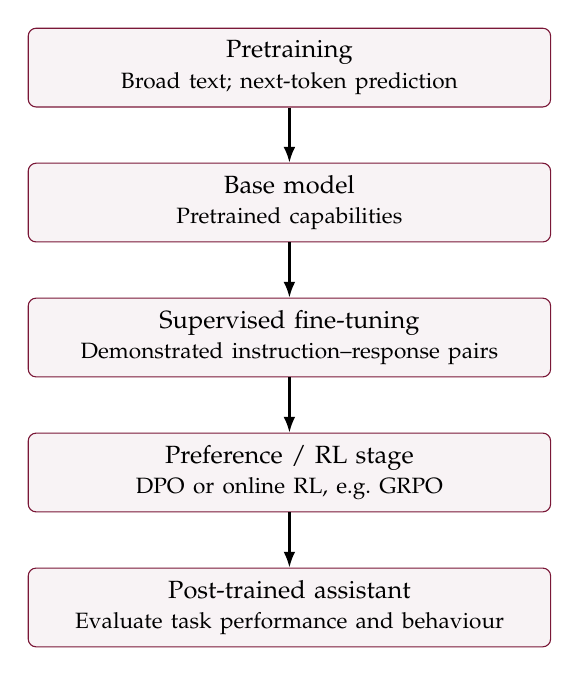
\begin{tikzpicture}[node distance=7mm]
\node[process,text width=64mm] (pre) {Pretraining\\\footnotesize Broad text; next-token prediction};
\node[process,text width=64mm,below=of pre] (base) {Base model\\\footnotesize Pretrained capabilities};
\node[process,text width=64mm,below=of base] (sft) {Supervised fine-tuning\\\footnotesize Demonstrated instruction--response pairs};
\node[process,text width=64mm,below=of sft] (pref) {Preference / RL stage\\\footnotesize DPO or online RL, e.g.\ GRPO};
\node[process,text width=64mm,below=of pref] (final) {Post-trained assistant\\\footnotesize Evaluate task performance and behaviour};
\draw[arr] (pre)--(base);
\draw[arr] (base)--(sft);
\draw[arr] (sft)--(pref);
\draw[arr] (pref)--(final);
\end{tikzpicture}
\caption{A typical combined workflow, shown in chronological order. Pretraining produces the base model; SFT and preference/RL training are subsequent stages. R1-Zero deliberately skips SFT, and other workflows can repeat stages.}\label{fig:llmpipeline}
\end{figure}\FloatBarrier
The source's arrow marked ``Pre-Training / Knowledge Injection'' is placed between ``Base Model'' and ``SFT Phase''. The redraw clarifies the chronology: a base model is the product of pretraining, and SFT then adapts it. The figure separates processes from resulting checkpoints and gives the preference/RL step its own node.

SFT supports rapid task adaptation, consistent response structure, and specific tool-call syntax. RL can search for effective strategies and improve reward-measured reasoning beyond the supplied demonstrations. Reducing hallucinations and improving adherence to safety guidelines are possible goals, not automatic consequences of using RL. The source's comparison to human demonstrator speed describes an ambition for scalable training, not a proven general speed advantage.

\subsection{Key takeaways and literature route}\label{sec:llmtakeaways}
Track four objects separately: the trainable policy, its fixed reference, the old sampling policy, and any reward model. A likelihood target, a human preference, and a rule-based correctness reward are different supervision signals. Distinguish the intended objective from the surrogate used to optimize it, and distinguish experimental improvements from guarantees.

The lecture's reading list moves from FLAN and LIMA (instruction tuning), to InstructGPT and DPO (human preferences), to DeepSeekMath, DeepSeek-V3, and DeepSeek-R1 (GRPO and reasoning). Sutton and Barto supply the foundations of Markov decision processes, value functions, and policy gradients; Jurafsky and Martin cover language-model architectures and training. Full entries for every cited paper and both books appear in Appendix~\ref{app:llmrefs}.

\clearpage
\section{Quick review}
\begingroup\small
\subsection{Core distinctions}
\begin{center}\small
\begin{tabularx}{\textwidth}{@{}P{39mm}Y@{}}\toprule
Question & What to check\\\midrule
What is the state? & Variables sufficient to propagate the model, not necessarily just the output.\\\addlinespace
What does the input affect? & Next frame or next sample; do not shift input/measurement pairs.\\\addlinespace
Is a model exact? & Separate assumed plant structure, learned parameters, exact sampling, and approximations.\\\addlinespace
Is the system stable? & Continuous LTI: $\operatorname{Re}\lambda_i<0$. Discrete LTI: $|\lambda_i|<1$.\\\addlinespace
Is it optimal? & PMP supplies necessary conditions; Bellman/HJB characterize optimal future cost under their assumptions.\\\addlinespace
What runs backward? & Costates, value functions, and finite-horizon Riccati equations.\\\addlinespace
What supervises the LLM? & Demonstrated targets (SFT), pairwise preferences (DPO/RLHF), or scores on generated outputs (online RL).\\\addlinespace
Which policy is fixed? & Distinguish the reference policy from the old sampling policy; both differ from the trainable policy.\\\bottomrule
\end{tabularx}\end{center}

\subsection{Exam revision prompts}
\begin{enumerate}
\item Derive the sliding-window gain estimate and state exactly when its denominator vanishes.
\item Starting from the two compressor state equations, compute the determinant and explain why one pole is zero.
\item Explain why $K=(1-p)/\widehat\alpha$ places a nominal pole but does not establish an unconditional adaptive guarantee.
\item Derive both Euler and exact ZOH motor updates. Identify the missing damping term in the source's approximate displacement.
\item Explain the transpose in PageRank and why a stationary eigenvalue $1$ is compatible with convergence of probability distributions.
\item State the continuous and discrete stability criteria, and derive the Lyapunov energy decrement.
\item Derive the adjoint equations using the correct sign or index for each time domain.
\item Starting from Bellman's equation, derive the DLQR gain and explain the use of $P_{k+1}$.
\item State the SFT, reward-model, and DPO losses, with datasets and trainable parameters.
\item Explain KL between distributions and the sampled log-ratio form of the RLHF objective.
\item Compute group-normalized advantages, including the equal-reward case.
\item Contrast clipping with hard constraints, and R1-Zero with the four-stage R1 workflow.
\end{enumerate}

\subsection{Compact terminology}
\textbf{Plant:} controlled environment or process. \textbf{Reference:} desired output. \textbf{Feedback:} use of measured behaviour in selecting inputs. \textbf{Online identification:} model estimation during operation. \textbf{Equilibrium:} constant state under a compatible constant input. \textbf{Schur stable:} all eigenvalues strictly inside the unit disk. \textbf{Costate:} adjoint multiplier for dynamic constraints. \textbf{Value function:} optimal remaining cost. \textbf{Riccati equation:} matrix equation governing a quadratic value function in LQR. \textbf{ZOH:} input held constant between samples. \textbf{SFT:} supervised fine-tuning on demonstrated responses. \textbf{RLHF:} reinforcement learning from human feedback. \textbf{DPO:} direct preference optimization. \textbf{GRPO:} group relative policy optimization. \textbf{CoT:} chain of thought. \textbf{KL divergence:} a directional measure of distribution mismatch.

\par\endgroup
\appendix
\clearpage
\section{Corrections and source ambiguities}\label{app:corrections}
This register records substantive changes and assumptions. Spelling and malformed slide totals have been normalized without changing academic content. Additional derivations are identified in the main text.

\begin{longtable}{@{}P{33mm}P{116mm}@{}}
\toprule Source & Treatment in these notes\\\midrule\endhead
Introduction p.\ 3 & The registration instruction names ``Software Verification''. Preserved as an unresolved course-name mismatch. Timetable and assessment are reported as source information.\\\addlinespace
Compressor p.\ 3 & The $[0,1]$ SSIM scale is retained as the case-study convention, not a universal range for general SSIM. The orientation and feasible range of the compressor setting are unspecified.\\\addlinespace
Compressor pp.\ 8--10 & The displayed objective is a sum, not a mean, of squared errors. Both have the same minimizer. A nonzero input-energy denominator is required.\\\addlinespace
Compressor pp.\ 11--12 & The stated control law is integral-only despite the PI label. The sum identity assumes a fixed gain.\\\addlinespace
Compressor pp.\ 20--24 & The characteristic polynomial has zero constant term. Correct poles: $0$ and $1-\alpha K$. The original erroneous two-pole argument is explicitly reconstructed and diagnosed in \cref{sec:sourcepoles}; its interval reparameterization is also invalid. The final gain formula remains valid by the corrected derivation.\\\addlinespace
Compressor pp.\ 23--27 & The estimate is distinguished from the true gain. Fixed-model pole placement is not a general adaptive-stability proof. Warm-up settings and accumulator treatment are unspecified; the learner also needs past control settings.\\\addlinespace
Continuous systems p.\ 5 & Lyapunov stability means remaining close, not merely bounded. Asymptotic stability includes stability plus attraction. Controllability is qualified by admissible-input constraints.\\\addlinespace
Continuous systems p.\ 6 & The car model's five components are not fully specified. No fifth variable is invented. Non-holonomic is a motion constraint.\\\addlinespace
Discrete systems pp.\ 5--6 & Exact ZOH is separated from leading-order input approximations. A consistent second-order angle expansion includes damping. Constant held voltage does not generally mean constant acceleration.\\\addlinespace
Discrete systems pp.\ 7--8 & Stable age-profile convergence requires suitable matrix assumptions. Growth factor and normalized age distribution are distinguished.\\\addlinespace
Discrete systems pp.\ 9--10 & Dangling pages need stochastic rows before damping. Stationary PageRank is not stability of the origin in the full vector space.\\\addlinespace
Discrete systems p.\ 11 & $\mathcal R_0$ describes initial growth; later growth depends on $S_k$. Parameter scaling and nonnegative-step conditions are clarified.\\\addlinespace
Discrete systems pp.\ 12--14 & Exact-sampling stability differs from Euler stability. Lyapunov strict inequalities exclude zero. The open-loop motor has an angle integrator. Taxonomy interventions are not present in the displayed models.\\\addlinespace
Continuous optimal control pp.\ 2--4, 6 & Normality, smoothness, admissibility, and endpoint assumptions are made explicit. Necessary PMP conditions are distinguished from HJB verification. State constraints are not universally easy to handle.\\\addlinespace
Both LQR slides, p.\ 5 & Standard definiteness assumptions and unconstrained inputs are stated. Riccati signs, terminal conditions, and discrete $k+1$ indexing are preserved.\\\addlinespace
Discrete optimal control pp.\ 2--4 & Zero-gradient stationarity requires an interior/unconstrained input. A terminal set changes the boundary condition. Finite-horizon backward recursion is distinguished from infinite-horizon value iteration.\\\addlinespace
LLM p.\ 4 & Output masking removes prompt-position losses, not all gradient paths through prompt representations. Dataset scales are illustrative.\\\addlinespace
LLM p.\ 5 & Vicuna's count denotes conversations. LIMA supports a hypothesis experimentally; it does not prove that SFT only teaches style.\\\addlinespace
LLM pp.\ 7--8 & KL acts on response distributions. The RLHF objective is distinguished from PPO's algorithm; offline DPO is separated from online exploration. Mixtral-8x22B's DPO attribution is not established by the reviewed official card.\\\addlinespace
LLM p.\ 9 & Distinct normalization and clipping constants are used. The source expression is identified as a sampled clipped surrogate that omits the training expectation and KL penalty. Equal group rewards give zero advantages.\\\addlinespace
LLM p.\ 10 & R1's later SFT mixture is approximately 600k reasoning plus 200k general samples. Final RL combines rule-based and learned reward signals.\\\addlinespace
LLM pp.\ 11--12 & ``Zero/high'' exploration and ``medium/high'' reasoning are qualified; no universal capability bound follows. The diagram places pretraining before the base checkpoint. Training goals are not guarantees.\\\addlinespace
LLM p.\ 15 & Jurafsky--Martin's 2024 citation is treated as a third-edition draft; chapter numbers vary with the draft.\\\bottomrule
\end{longtable}

\Needspace{10\baselineskip}
\section{Source coverage map}\label{app:coverage}
Every physical source page is accounted for below. Title and closing pages are tracked separately from academic content. Repeated derivation steps are consolidated without losing their equations or conclusions. The compressor architectures are redrawn in \cref{fig:compressor,fig:abstract,fig:adaptive}; the LLM training pipeline is redrawn in \cref{fig:llmpipeline}. Equations and comparison tables are typeset directly. Current optimal-control filenames replace their identical earlier aliases, without duplicating source-page counts.

\small
\begin{longtable}{@{}P{29mm}P{14mm}P{105mm}@{}}
\toprule File & Page & Content destination\\\midrule\endhead
1000-\allowbreak intro & 1 & Title page; course identity in Section 1.1.\\
 & 2 & Section 1.1: timetable, room, address.\\
 & 3 & Section 1.1: platform, recordings, registration ambiguity, contact.\\
 & 4 & Section 1.1: assessment weights and individual pass thresholds.\\
 & 5 & Section 1.1: full course-material list.\\
 & 6 & Section 1.2: all four objectives.\\
 & 7 & Section 1.2: closing acknowledgement; no additional content.\\
\addlinespace
1500-\allowbreak video-\allowbreak compressor & 1 & Section 2 opening and 2.1: title, identity, research URL.\\
 & 2 & Section 2.1: full case-study reference.\\
 & 3 & Section 2.1: bandwidth--quality trade-off, SSIM, image dependence.\\
 & 4 & Section 2.2 and Figure 2.1: detailed plant and online learning.\\
 & 5 & Section 2.2 and Figure 2.2: abstract plant and planning.\\
 & 6 & Section 2.3 and Figure 2.2: signal timing and plant equation.\\
 & 7 & Section 2.3: reference 0.9 and parameter-learning rationale.\\
 & 8 & Section 2.4: sliding-window measurements, predictions, objective.\\
 & 9 & Section 2.4: all derivative steps and stationarity.\\
 & 10 & Section 2.4: estimator and known-quantity interpretation.\\
 & 11 & Section 2.5: error, integral law, positive gain, PI terminology.\\
 & 12 & Section 2.5: accumulator, initialization, sum identity.\\
 & 13 & Sections 2.5--2.6: closed loop and input recurrence.\\
 & 14 & Section 2.6: error-based and reference-based state equations.\\
 & 15 & Section 2.6: expanded two-state equations.\\
 & 16 & Sections 2.6--2.7: tracking and asymptotic-stability design goals.\\
 & 17 & Section 2.6: equilibrium substitutions.\\
 & 18 & Section 2.6: equilibrium solution and regulator interpretation.\\
 & 19 & Sections 2.6--2.7: system matrix and eigenvalue criterion.\\
 & 20 & Sections 2.7--2.8: determinant, corrected polynomial, source error.\\
 & 21 & Section 2.8: original coefficient comparison and missing factor.\\
 & 22 & Section 2.8: original pole relation, with its invalid premise.\\
 & 23 & Sections 2.7--2.8: source gain and model-scaling interpretation.\\
 & 24 & Sections 2.7--2.8: reparameterization flaw; valid final gain.\\
 & 25 & Section 2.7: all expanded and error-based final dynamics.\\
 & 26 & Section 2.9: full learning/control update and warm-up assumptions.\\
 & 27 & Section 2.9 and Figure 2.3: revised intelligent-system boundary.\\
 & 28 & Closing acknowledgement only; no new academic content.\\
\addlinespace
2000-\allowbreak ct-\allowbreak systems & 1 & Section 3 opening: title, subtitle, lecturer attribution, date.\\
 & 2 & Section 3.1: nonlinear and LTI models, variables and dimensions.\\
 & 3 & Section 3.2: quadrotor state, inputs, four motion equations.\\
 & 4 & Section 3.3: manipulator model and first-order conversion.\\
 & 5 & Section 3.4: equilibrium, stability, eigenvalues, controllability.\\
 & 6 & Section 3.5: every row and column of the taxonomy.\\
\addlinespace
3000-\allowbreak dt-\allowbreak systems & 1 & Section 4 opening and reading guide: title, subtitle, date, attribution.\\
 & 2 & Section 4.1: nonlinear and LTI difference equations.\\
 & 3 & Section 4.1: sampling, digital motivation, recursive predictions.\\
 & 4 & Section 4.2: motor, Euler derivation and matrices.\\
 & 5 & Sections 4.3--4.4: ZOH velocity, both integrals and Taylor expansion.\\
 & 6 & Section 4.4: input matrices, within-step displacement, corrections.\\
 & 7 & Section 4.5: Leslie state, matrix, fecundity, survival.\\
 & 8 & Section 4.5: births, aging, three eigenvalue cases and assumptions.\\
 & 9 & Section 4.6: random surfer, row-stochastic matrix, transpose.\\
 & 10 & Section 4.6: damping 0.85/0.15, stationary distribution, iteration.\\
 & 11 & Section 4.7: all SIR equations, parameters, reproduction condition.\\
 & 12 & Section 4.8: Schur criterion and exact eigenvalue mapping.\\
 & 13 & Section 4.9: Lyapunov equation and energy decrement.\\
 & 14 & Section 4.10: full taxonomy and limits of its criteria.\\
\addlinespace
1000-\allowbreak opt-\allowbreak ctr-\allowbreak ct-\allowbreak sys & 1 & Section 5 opening: title, subtitle, lecturer, date.\\
 & 2 & Section 5.1: objective, dynamics, inputs, terminal set and time.\\
 & 3 & Section 5.2: Hamiltonian, state, adjoint, minimization, transversality.\\
 & 4 & Section 5.3: value function, HJB, boundary, feedback.\\
 & 5 & Section 5.4: LQR cost, stationarity, ansatz, Riccati, gain.\\
 & 6 & Section 5.5: all five comparison dimensions, with qualifications.\\
\addlinespace
2000-\allowbreak opt-\allowbreak ctr-\allowbreak dt-\allowbreak sys & 1 & Section 6 opening: title, subtitle, lecturer, date.\\
 & 2 & Section 6.1: horizon, objective, dynamics, inputs, terminal set.\\
 & 3 & Section 6.2: Hamiltonian and four necessary conditions.\\
 & 4 & Section 6.3: value function, Bellman equation, boundary, feedback.\\
 & 5 & Section 6.4: DLQR cost, gain, Riccati, terminal matrix.\\
 & 6 & Section 6.5: all six continuous/discrete comparison dimensions.\\
\addlinespace
3000-\allowbreak RL4LLM & 1 & Section 7 opening: full title, subtitle, lecturer, overview, date.\\
 & 2 & Section 7 opening and 7.10: all four agenda themes.\\
 & 3 & Section 7.1: pretraining, SFT role, original prompt and target fragment.\\
 & 4 & Section 7.1: autoregressive loss, masking, scale and data sources.\\
 & 5 & Section 7.2: Alpaca, Vicuna, LIMA and the hypothesis qualification.\\
 & 6 & Section 7.3: multiple answers, sequence rewards, exploration.\\
 & 7 & Section 7.4: three RLHF stages, Bradley--Terry loss, KL objective.\\
 & 8 & Section 7.5: DPO loss, implicit reward, all adoption examples.\\
 & 9 & Section 7.6: R1-Zero, all group statistics, clipped surrogate, behaviour.\\
 & 10 & Section 7.7: all four R1 stages, readability and language mixing.\\
 & 11 & Section 7.8: all six comparison rows, with explicit qualifications.\\
 & 12 & Section 7.9 and Figure 7.1: pipeline, examples, SFT and RL roles.\\
 & 13 & Section 7.10 and Appendix C.3: FLAN, LIMA, InstructGPT, DPO.\\
 & 14 & Section 7.10 and Appendix C.3: DeepSeekMath, V3, R1.\\
 & 15 & Section 7.10 and Appendix C.3: both textbooks and reading scope.\\
\bottomrule\end{longtable}\normalsize

\clearpage
\section{References and compilation}\label{app:references}
\subsection{Primary lecture material}
All academic topics are grounded in the following supplied PDFs:
\begin{itemize}
\item \texttt{1000-intro.pdf}
\item \texttt{1500-video-compressor.pdf}
\item \texttt{2000-ct-systems.pdf}
\item \texttt{3000-dt-systems.pdf}
\item \texttt{1000-opt-ctr-ct-sys.pdf}
\item \texttt{2000-opt-ctr-dt-sys.pdf}
\item \texttt{3000-RL4LLM.pdf}
\end{itemize}
The supplied \emph{Biometric Systems} PDF was used only as a visual reference.

\subsection{Reference cited by the lecture}
Antonio Filieri, Henry Hoffmann, and Martina Maggio. \emph{Automated design of self-adaptive software with control-theoretical formal guarantees}. Proceedings of the 36th International Conference on Software Engineering (ICSE 2014), ACM, New York, NY, USA, pp.\ 299--310. \href{https://doi.org/10.1145/2568225.2568272}{doi:10.1145/2568225.2568272}.

\subsection{Literature cited by the LLM lecture}\label{app:llmrefs}
The following seven papers and two books reproduce the complete reading list on source pages 13--15. Dates refer to the versions or publication years cited by the lecture.
\begin{enumerate}
\item Jason Wei et al.\ (2021). \emph{Finetuned Language Models Are Zero-Shot Learners}. ICLR 2022. FLAN and instruction tuning. \href{https://arxiv.org/abs/2109.01652}{arXiv:2109.01652}.
\item Chunting Zhou et al.\ (2023). \emph{LIMA: Less Is More for Alignment}. NeurIPS 2023. Data-efficient SFT and the alignment hypothesis. \href{https://arxiv.org/abs/2305.11206}{arXiv:2305.11206}.
\item Long Ouyang et al.\ (2022). \emph{Training language models to follow instructions with human feedback}. NeurIPS 2022. InstructGPT and the SFT--reward-model--PPO workflow. \href{https://arxiv.org/abs/2203.02155}{arXiv:2203.02155}.
\item Rafael Rafailov et al.\ (2023). \emph{Direct Preference Optimization: Your Language Model is Secretly a Reward Model}. NeurIPS 2023. Preference loss and implicit reward reparameterization. \href{https://arxiv.org/abs/2305.18290}{arXiv:2305.18290}.
\item Zhihong Shao et al.\ (2024). \emph{DeepSeekMath: Pushing the Limits of Mathematical Reasoning in Open Language Models}. Introduces GRPO. \href{https://arxiv.org/abs/2402.03300}{arXiv:2402.03300}.
\item DeepSeek-AI (2024). \emph{DeepSeek-V3 Technical Report}. Mixture-of-Experts (MoE) architecture and GRPO post-training. \href{https://arxiv.org/abs/2412.19437}{arXiv:2412.19437}.
\item DeepSeek-AI (2025). \emph{DeepSeek-R1: Incentivizing Reasoning Capability in LLMs via Reinforcement Learning}. R1-Zero and the hybrid R1 workflow. Technical checks here use the original report, version 1. \href{https://arxiv.org/abs/2501.12948v1}{arXiv:2501.12948v1}.
\item Richard S. Sutton and Andrew G. Barto (2018). \emph{Reinforcement Learning: An Introduction}. Second edition, MIT Press. Markov decision processes, value functions, and policy gradients.
\Needspace{5\baselineskip}
\item Dan Jurafsky and James H. Martin (2024 draft, as cited). \emph{Speech and Language Processing}. Third-edition draft; the slide recommends Chapters 10--13 for Transformers, fine-tuning, and alignment. Chapter numbering is draft-dependent: this is not a claim about every later revision.
\end{enumerate}

\subsection{Supplementary checks}
The references below support targeted technical checks; they do not replace the supplied course material.
\begin{itemize}
\item Zhou Wang, Alan C. Bovik, Hamid R. Sheikh, and Eero P. Simoncelli. \emph{Image quality assessment: From error visibility to structural similarity}. IEEE Transactions on Image Processing, vol.\ 13, no.\ 4, April 2004. Original paper: \href{https://www.cns.nyu.edu/pub/eero/wang03-reprint.pdf}{original SSIM paper}. Used to qualify the lecture's operational SSIM range.
\item Sanjay Lall, Stanford EE363. \emph{Linear quadratic regulator: Discrete-time finite horizon}. \href{https://ee363.stanford.edu/lectures/015_dlqr.pdf}{Stanford EE363 notes}. Used to cross-check the discrete Riccati recursion, gain, and definiteness assumptions.
\item Stanford EE363. \emph{Continuous time linear quadratic regulator}. \href{https://ee363.stanford.edu/lectures/018_clqr.pdf}{Stanford EE363 notes}. Used to cross-check the differential Riccati equation, feedback gain, and backward terminal-value formulation.
\end{itemize}
The compressor characteristic polynomial and motor discretization corrections follow directly from symbolic expansion and integration of the equations in the supplied slides. They do not depend on an alternate plant model.

\textbf{Additional primary checks for Section 7.} Historical counts were checked against Stanford CRFM's \emph{Alpaca} announcement (\href{https://crfm.stanford.edu/2023/03/13/alpaca.html}{Stanford CRFM Alpaca announcement}) and LMSYS's \emph{Vicuna} announcement (\href{https://lmsys.org/blog/2023-03-30-vicuna/}{LMSYS Vicuna announcement}). DPO attribution was checked against the Zephyr-7B-beta model card (\href{https://huggingface.co/HuggingFaceH4/zephyr-7b-beta}{Zephyr-7B-beta model card}) and Dubey et al., \emph{The Llama 3 Herd of Models} (2024), \href{https://arxiv.org/abs/2407.21783}{arXiv:2407.21783}. The official Mixtral-8x22B-Instruct-v0.1 card was reviewed without establishing the lecture's specific DPO attribution (\href{https://huggingface.co/mistralai/Mixtral-8x22B-Instruct-v0.1}{official Mixtral-8x22B-Instruct model card}); Mistral explicitly documents DPO for Mixtral-8x7B in \emph{Mixtral of experts} (\href{https://mistral.ai/news/mixtral-of-experts/}{Mistral, ``Mixtral of experts''}). The original DPO, LIMA, and R1 papers listed above support the corresponding mathematical and factual qualifications.

\subsection{Compiling the source}
Every diagram is written in TikZ; the cover uses the accompanying \texttt{assets/sapienza-logo.png} file. Run \texttt{build.ps1}, or compile with pdfLaTeX at least twice, to resolve the contents and cross-references. The source uses common TeX Live/MiKTeX packages, with Palatino text and matching mathematics, \texttt{microtype}, and reusable layout/box definitions. The \texttt{\% !TeX program = pdflatex} directive supports editor integration; VS Code's LaTeX Workshop must use an installed pdfLaTeX distribution.
\end{document}
